
In this chapter, we aim to characterise transcript degradation and read truncation from long-read RNA-seq data. Transcript degradation from the 5' end results in truncated reads and a decrease in coverage with increasing distance from the 3' end for a given isoform. Thus, even though the observed degradation occurs from the 5' end, it is helpful to characterise degradation as the resultant decrease in coverage from the 3' end. We formalize the notion of degradation by defining the \textit{degradation rate}. 
\begin{definition}[Normalized coverage]
Let the maximum coverage over an isoform be $\mathrm{cov}_{\mathrm{max}}$ and the coverage at base $b$ be $\mathrm{cov}_b$. The normalized coverage of the isoform at base $b$ is defined as 
\begin{equation}
    \mathrm{ncov}_b=\frac{\mathrm{cov}_b}{\mathrm{cov}_{\mathrm{max}}}
\end{equation}
\end{definition}
\begin{definition}[Degradation rate]
Let $\mathrm{ncov}$ be the normalized coverage over an isoform, and $x$ be the distance in kb from the 3' end. The degradation rate of an isoform is defined as the rate of change in normalized coverage with respect to distance in kb from the 3' end of the isoform:
\begin{equation}
    d=\lim_{\Delta x\rightarrow 0} \frac{\Delta \mathrm{ncov}}{\Delta x}
\end{equation}
The degradation rate of an isoform at a base $b$ with distance $x_b$ away from the 3' end is the value of this limit evaluated at $x=x_b$. 
\end{definition}
Intuitively, the degradation rate can be interpreted as the gradient of the plot of normalized coverage against distance from the 3' end. We will refer to this plot as the \textbf{degradation curve}. To illustrate this, we visualise degradation curves for a hypothetical isoform of length 2 kb with different degradation rates (Fig. \ref{fig:sec-2-hypo}).  
\begin{figure}[H]
    \centering
    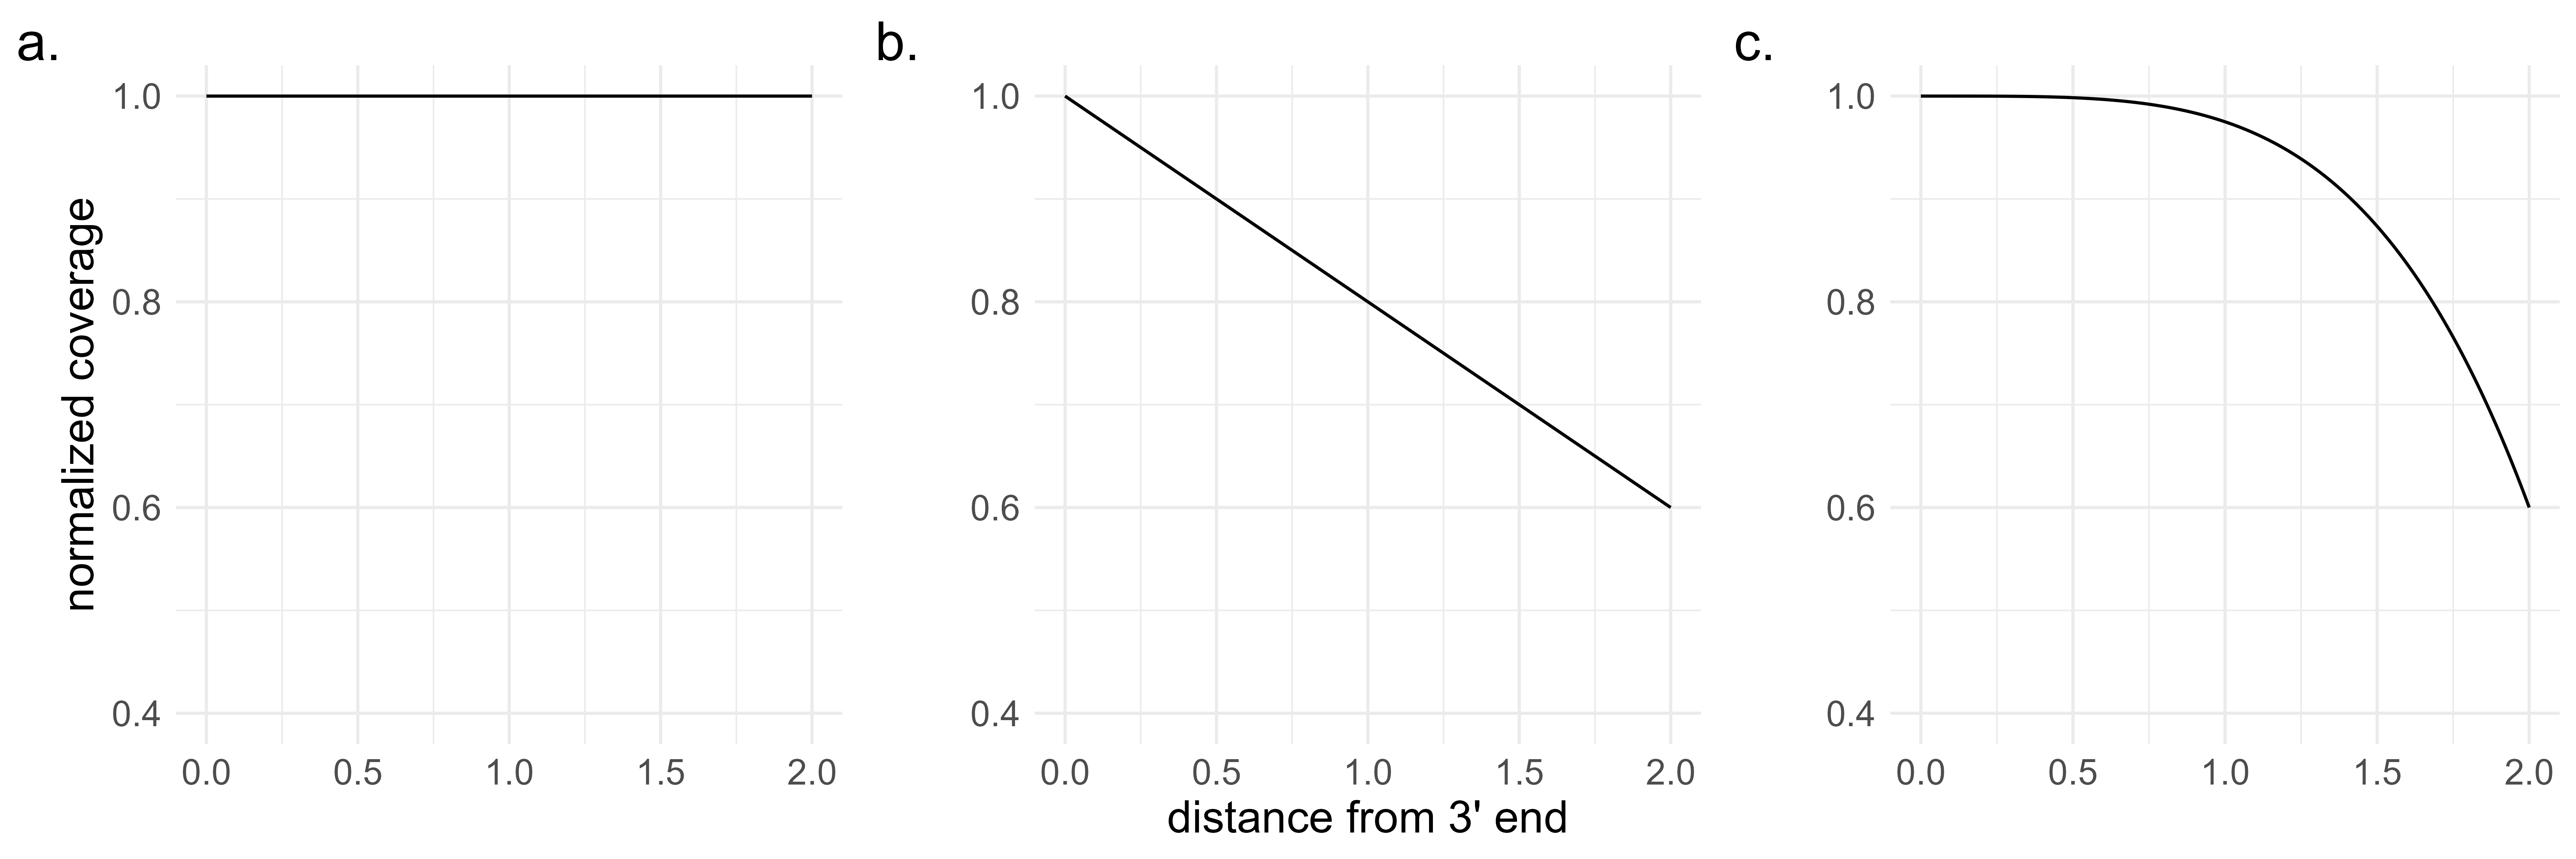
\includegraphics[width=\textwidth]{figures/sec-2-hypo.png}
    \caption[Normalized coverage plots for a hypothetical isoform]{Normalized coverage plots for a hypothetical isoform of length 2 kb illustrating different degradation rates. \textbf{a.} Degradation rate is 0. \textbf{b.} Degradation rate is constant (0.2). \textbf{c.} Degradation rate is variable.}
    \label{fig:sec-2-hypo}
\end{figure}
In Fig. \ref{fig:sec-2-hypo}a, the degradation rate or gradient is 0, implying that all reads from the isoform are full-length, with no drop in coverage over the isoform body. Conversely, in Fig. \ref{fig:sec-2-hypo}b, the gradient is a constant value of 0.2 over the isoform body, implying that for every 1 kb from the 3' end, normalized coverage drops by 0.2. The last plot in Fig. \ref{fig:sec-2-hypo}c shows variable gradient over the isoform body. In particular, the gradient is low in magnitude towards the 3' end and increases with distance from the 3' end.  

In the following sections, we first describe a coverage-based approach for characterising degradation in long-read direct RNA-seq data, and validate this approach with simulated data where the degradation is known. We then examine degradation in real data, characterising degradation by isoform features and in sequencing spike-ins. Finally, we develop a method for efficient read length-based degradation estimation that can be used for obtaining degradation-aware isoform abundance estimates.

\section{Coverage-based degradation estimation}\label{sec:deg-est}

We first sought to determine if patterns of degradation were consistent across transcript isoforms for a given direct RNA-seq dataset. To that end, we selected single-isoform, multi-exon genes from GRCh38 reference annotations, and further restricted the set of isoforms to those that do not intersect with any other annotated features in reference annotations. We refer to these as \textbf{lone isoforms}. Estimating bias from lone isoforms reduces ambiguity in the isoform of origin of the reads we use to estimate bias; such approaches were also adopted in \cite{Roberts2011} and \cite{Love2016} for bias estimation in short-read data. Filtering yielded approximately 5,000 lone isoforms. For each of these isoforms, we obtained coverage over the isoform body using the \texttt{genomecov} module from bedtools (v.2.27.1). Next, we further apply a median coverage filter, filtering out lone isoforms with low median coverage (min median coverage = 10). Finally, a degradation curve is fitted to the data with a smoothing spline.  

To validate this approach, we simulated two datasets where the expected degradation rates for all isoforms is constant ($\mathbb{E}[d]\in\{0.2,0.4\}$, see Appendix \ref{ap:sim-deg-reads} for more details on degraded read simulation). Visualising the degradation curves for each isoform, we observed noise in the form of deviation from the expected degradation curve (grey lines, Fig. \ref{fig:cov-sim}), likely due to sampling noise in the simulation data generation process. This noise can be mitigated by computing a global degradation curve across all isoforms (red line, Fig. \ref{fig:cov-sim}). We find that the global degradation curves reflect the known degradation rates from the simulated data qualitatively (Fig. \ref{fig:cov-sim}). In addition, we assessed the global degradation curves quantitatively by computing the average gradients of each curve, and found good agreement between the estimates and the expected degradation ($\mathbb{E}[d]$ = 0.2, estimated = 0.201; $\mathbb{E}[d]$ = 0.4, estimated = 0.403).

We applied this approach in real direct RNA-seq data from the SG-NEx project \cite{Chen2021}. Within each sample, we found consistent patterns of degradation across isoforms (Fig. \ref{fig:cov-real}). However, we note that for most real datasets, filtering for lone transcripts and by median coverage yields very few isoforms remaining for estimating degradation rates. For instance, in a HepG2 sample (Fig. \ref{fig:cov-real}a), we obtained only 57 isoforms, while in a MCF7 sample (Fig. \ref{fig:cov-real}b), we obtained only 52 isoforms. Across the samples, the median number of lone isoforms post-filtering was 21. While this approach separates signal and noise by considering only lone isoforms, it may be overly restrictive. We consider an improved approach for estimating the degradation rate in Section \ref{sec:rld} based on observed read length distributions. 

\begin{figure}[H]
    \centering
    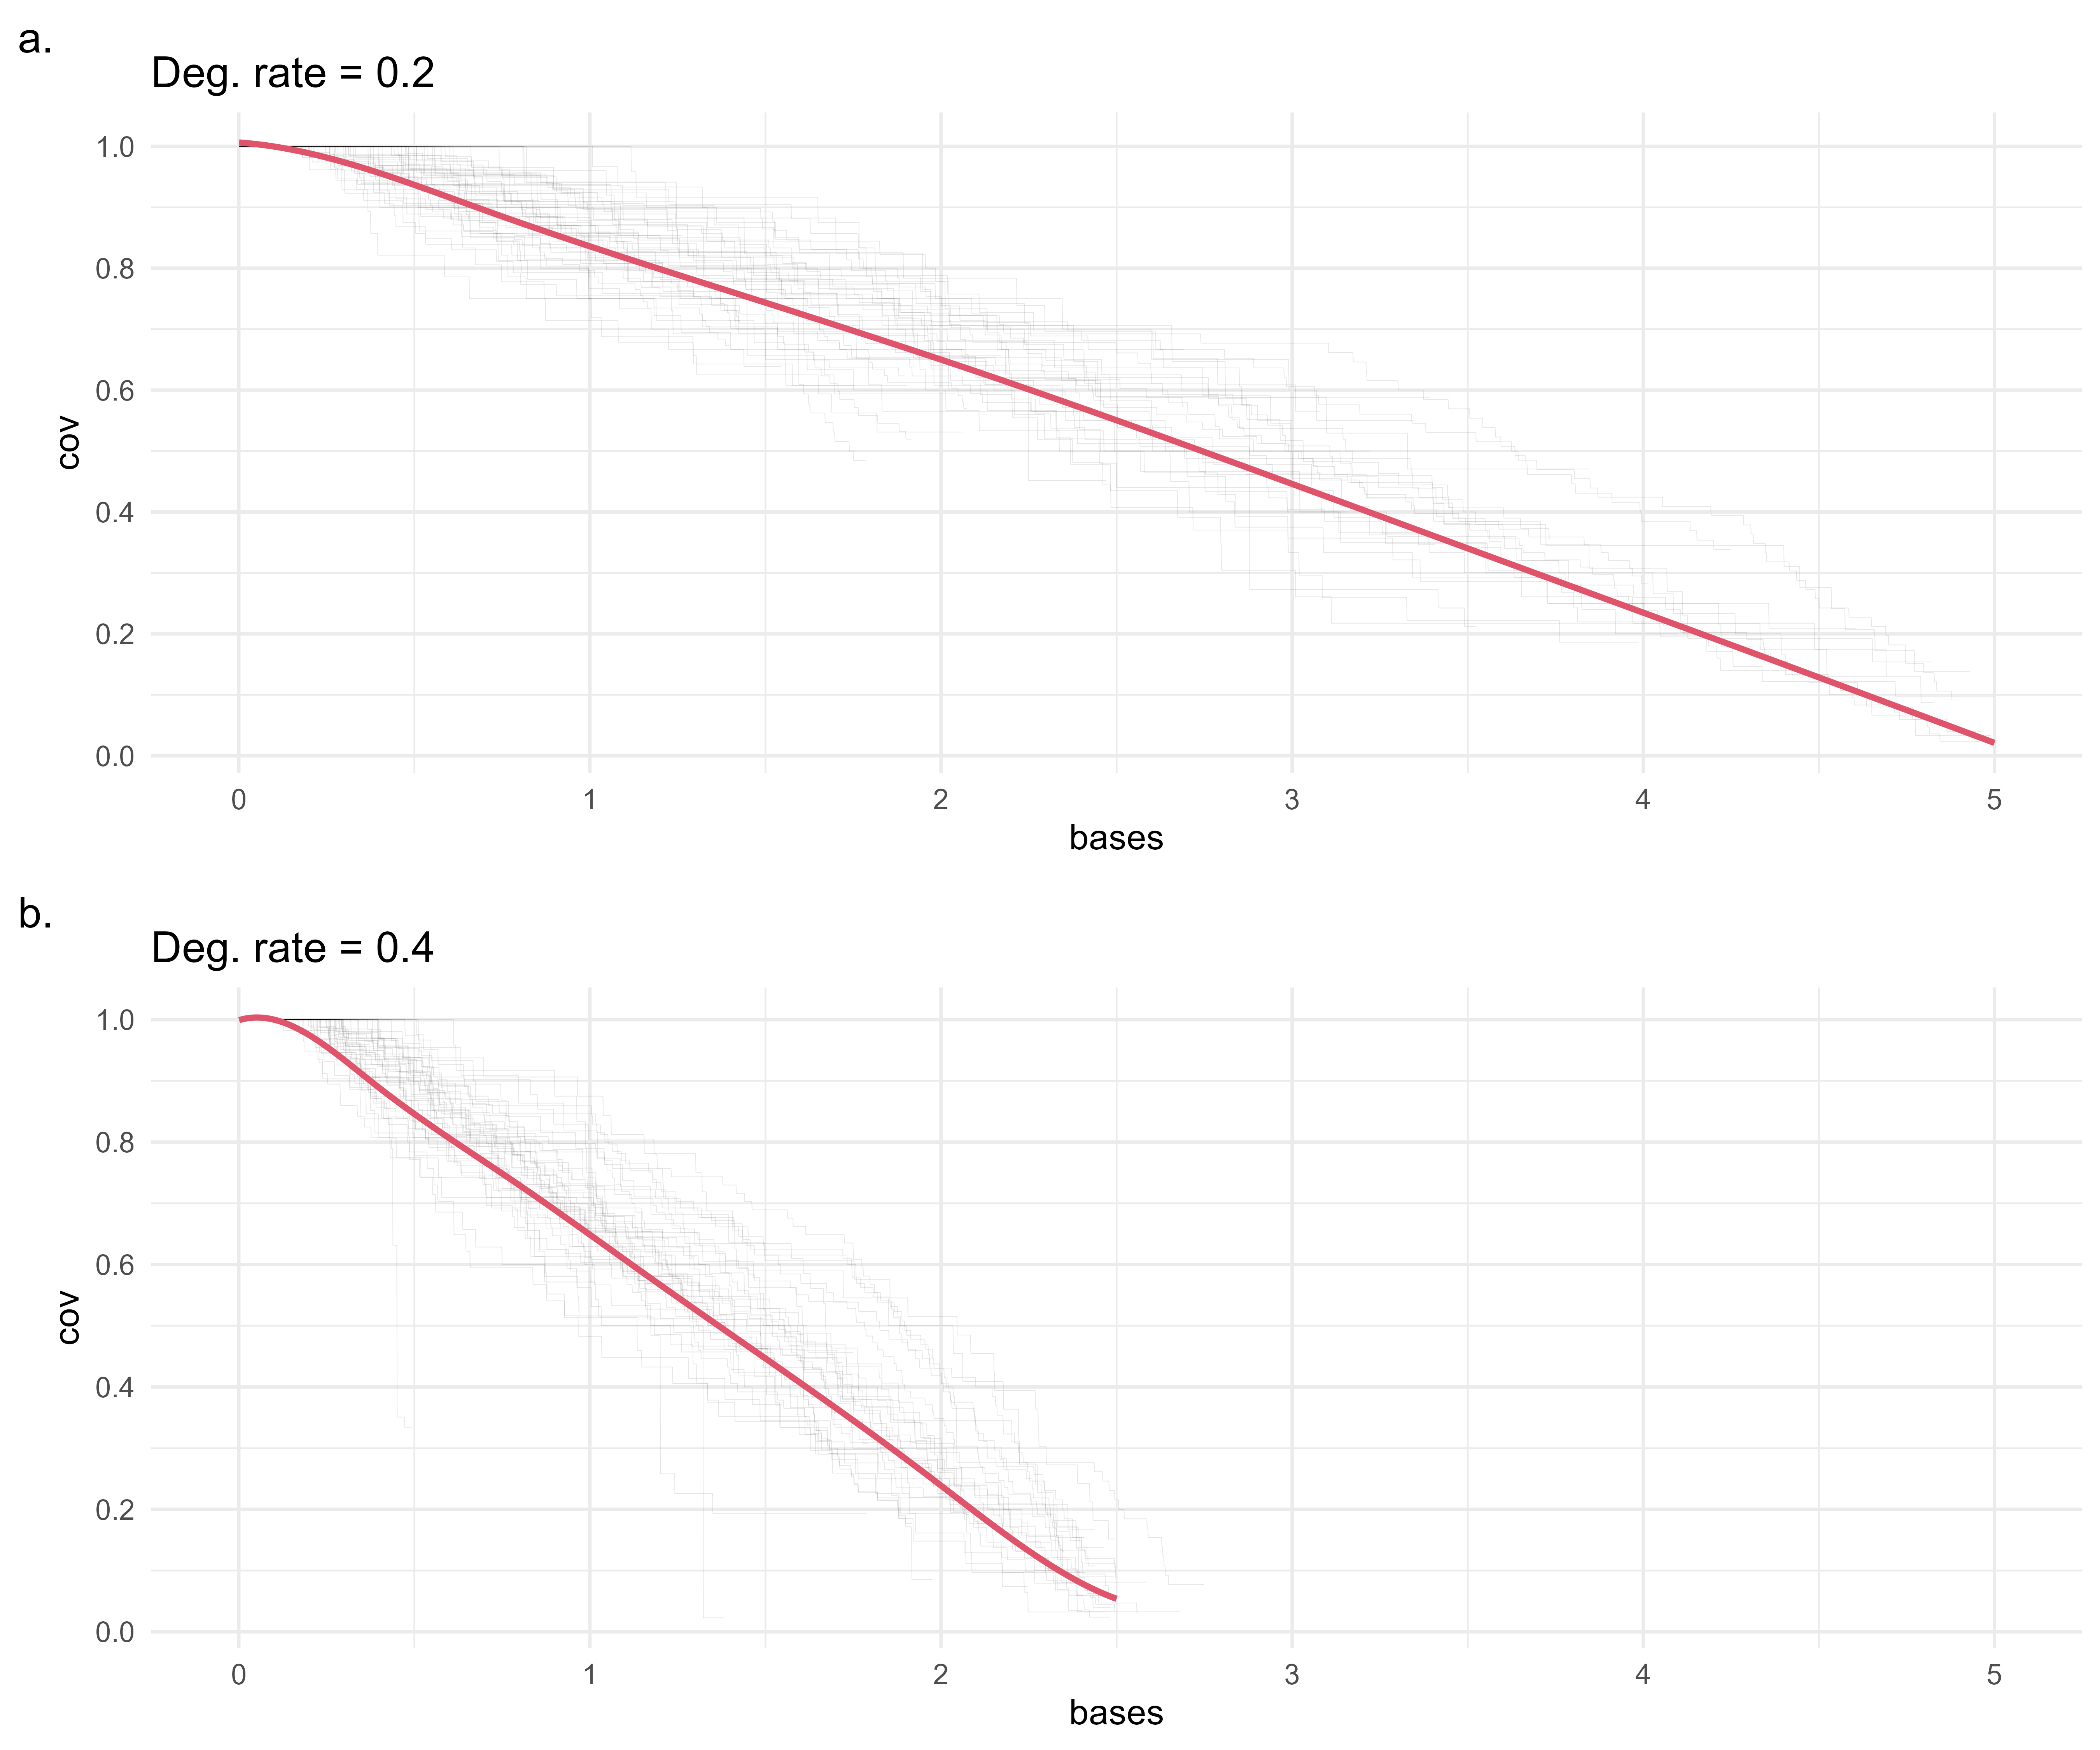
\includegraphics[width=0.9\textwidth]{figures/sec-2-cov-sim.png}
    \caption[Degradation curves on simulation datasets based on coverage]{Degradation curves on simulation datasets based on coverage. Grey translucent lines represent the coverage curves for individual isoforms. The red line represents the spline fitted across all isoforms. \textbf{a.} Degradation curve for dataset with $\mathbb{E}[d]$ = 0.2. Coverage drops close to 0 at 5kb with a degradation rate of 0.2. The estimated degradation rate is 0.201. \textbf{a.} Degradation curve for dataset with $\mathbb{E}[d]$ = 0.4. Coverage drops close to 0 at 2.5 kb. The estimated degradation rate is 0.403.}
    \label{fig:cov-sim}
\end{figure}

\begin{figure}[H]
    \centering
    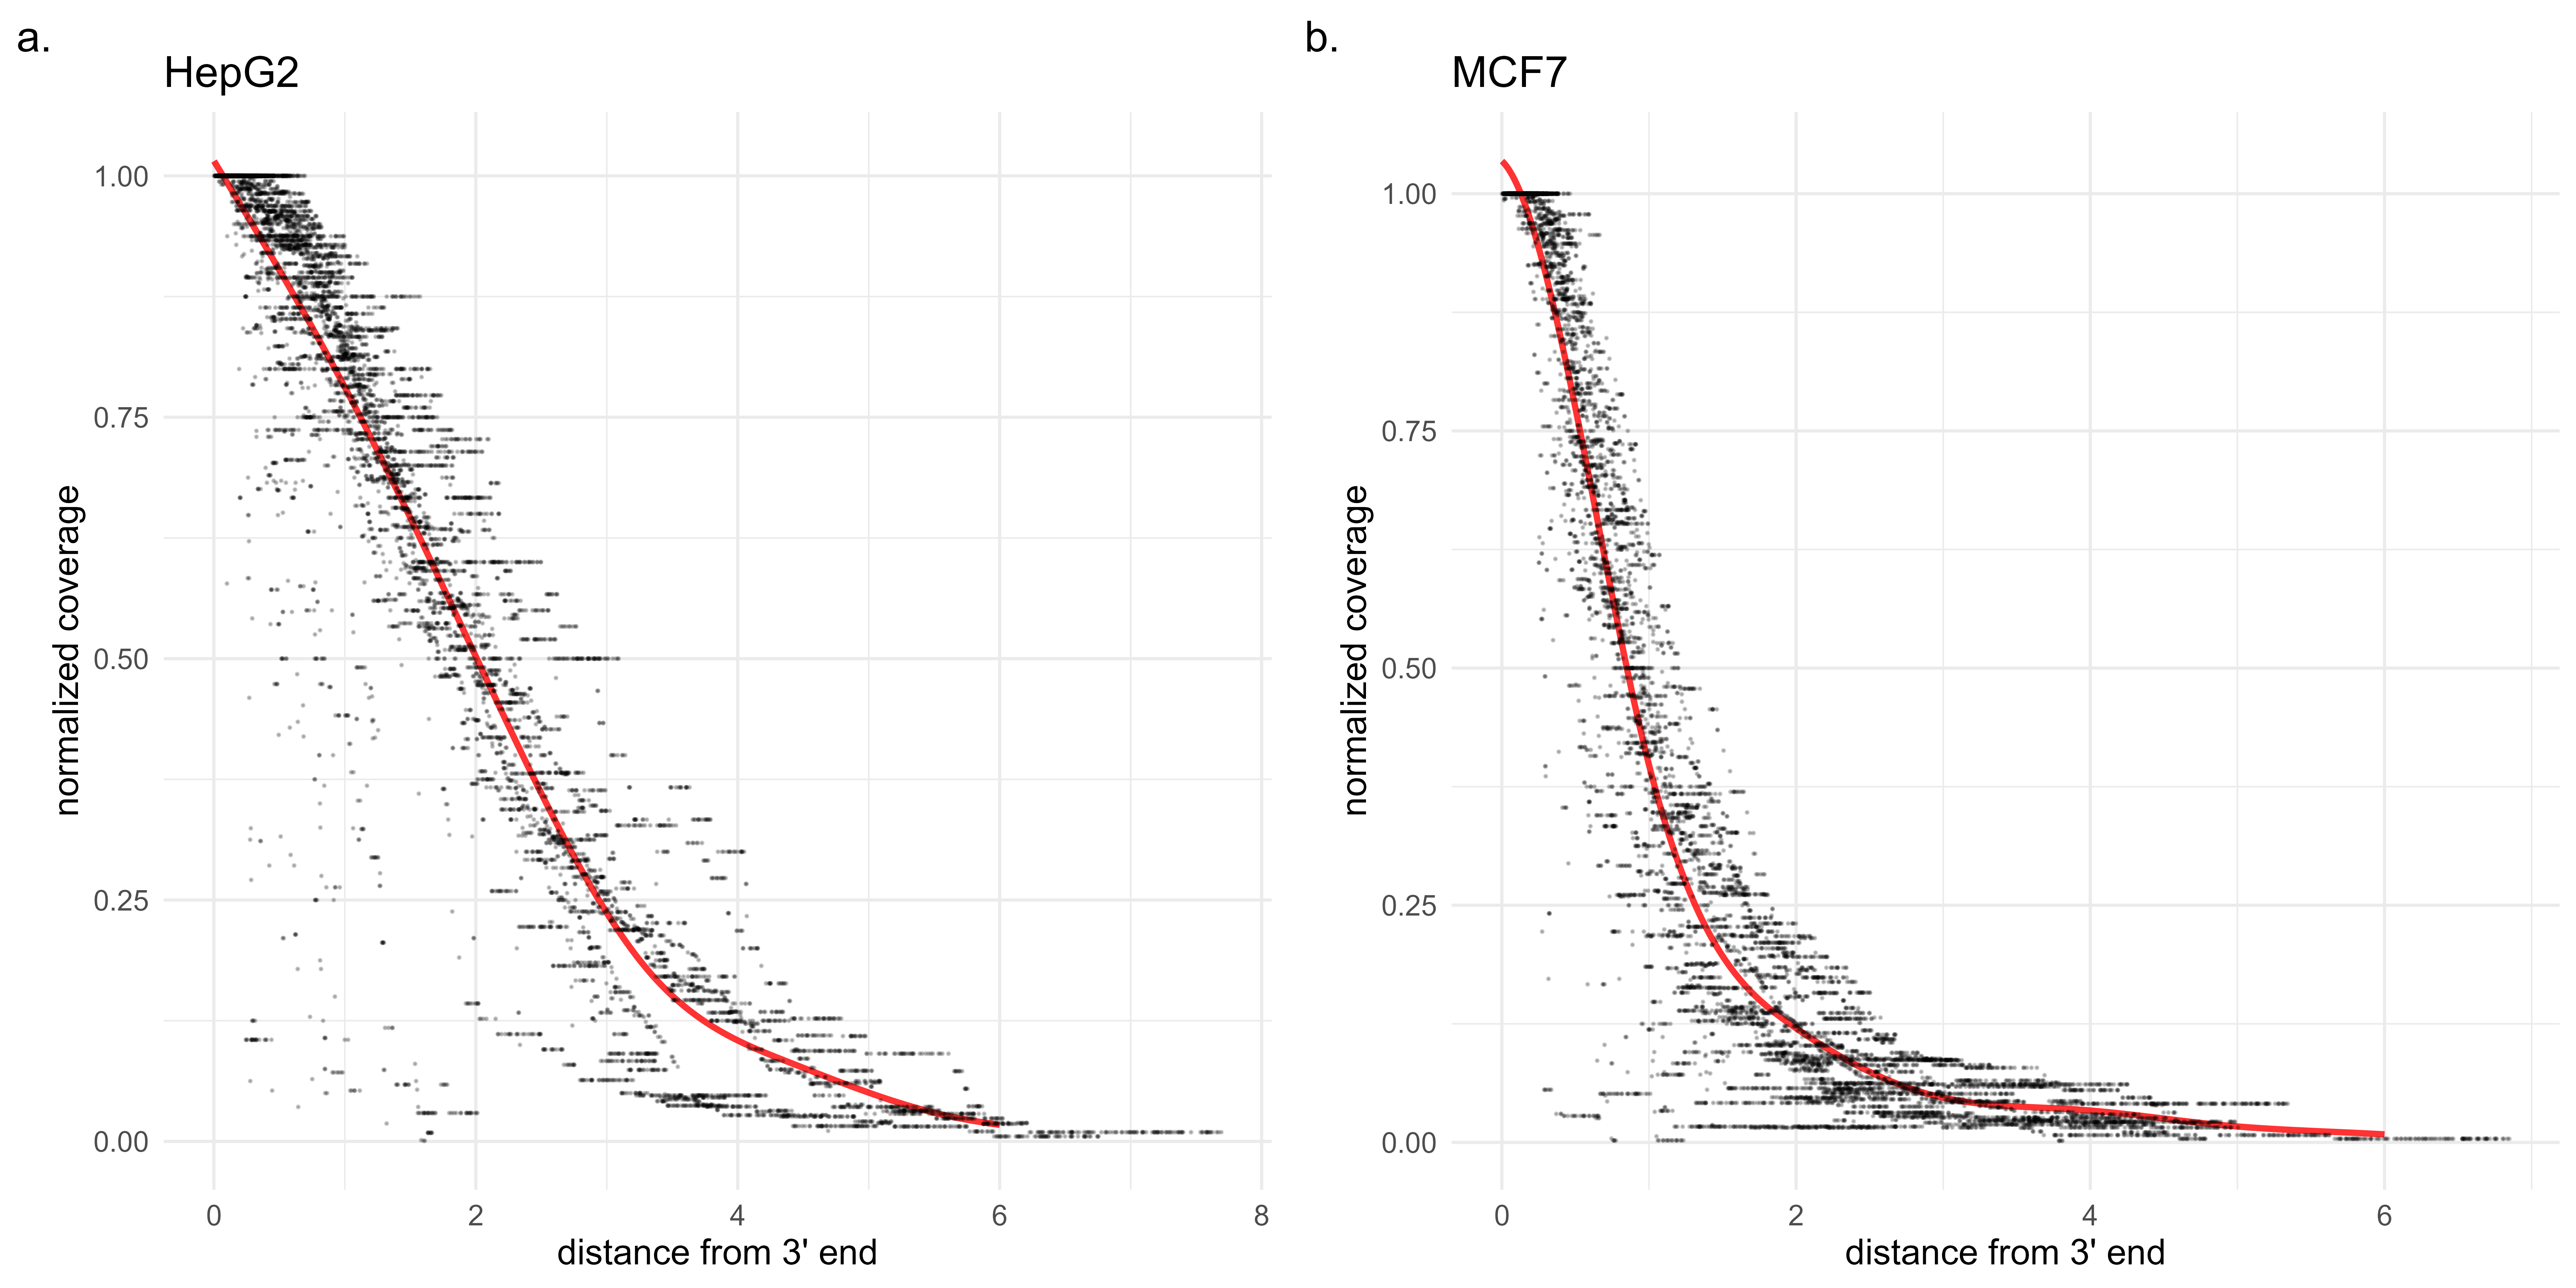
\includegraphics[width=0.9\textwidth]{figures/sec-2-cov-real.png}
    \caption[Degradation curves on real datasets based on coverage]{Degradation curves on real datasets based on coverage. Grey translucent lines represent the coverage curves for individual isoforms. The red line represents the spline fitted across all isoforms. These two datasets had the most number of isoforms post-filtering for degradation rate estimation (n = 57, 52). \textbf{a.} Degradation curve for a HepG2 cell line sample. \textbf{b.} Degradation curve for a MCF7 cell line sample.}
    \label{fig:cov-real}
\end{figure}

\subsection{Degradation by isoform features}

Here, we explore whether degradation rates vary between isoforms of different features. In particular, we striate isoforms by their annotated length (Fig. \ref{fig:cov-feature}a), observed median coverage (Fig. \ref{fig:cov-feature}b) and biotype (Fig. \ref{fig:cov-feature}c). On a representative sample from the MCF7 cell line, estimated degradation rates do not appear to vary significantly between isoforms of different annotated length or median coverage (Fig. \ref{fig:cov-feature}a,b). However, the converse is true for different transcript biotypes. In particular, we observe higher degradation rates for processed pseudogenes (n = 7) and long non-coding RNAs (n = 3) as compared to protein coding genes (n = 42, Fig. \ref{fig:cov-feature}c). While the sample size here is small, this result corroborates findings in \cite{Clark2012} and \cite{Kaiwan2021}, which identified larger variance in the stabilities of lncRNAs.   

\begin{figure}[H]
    \centering
    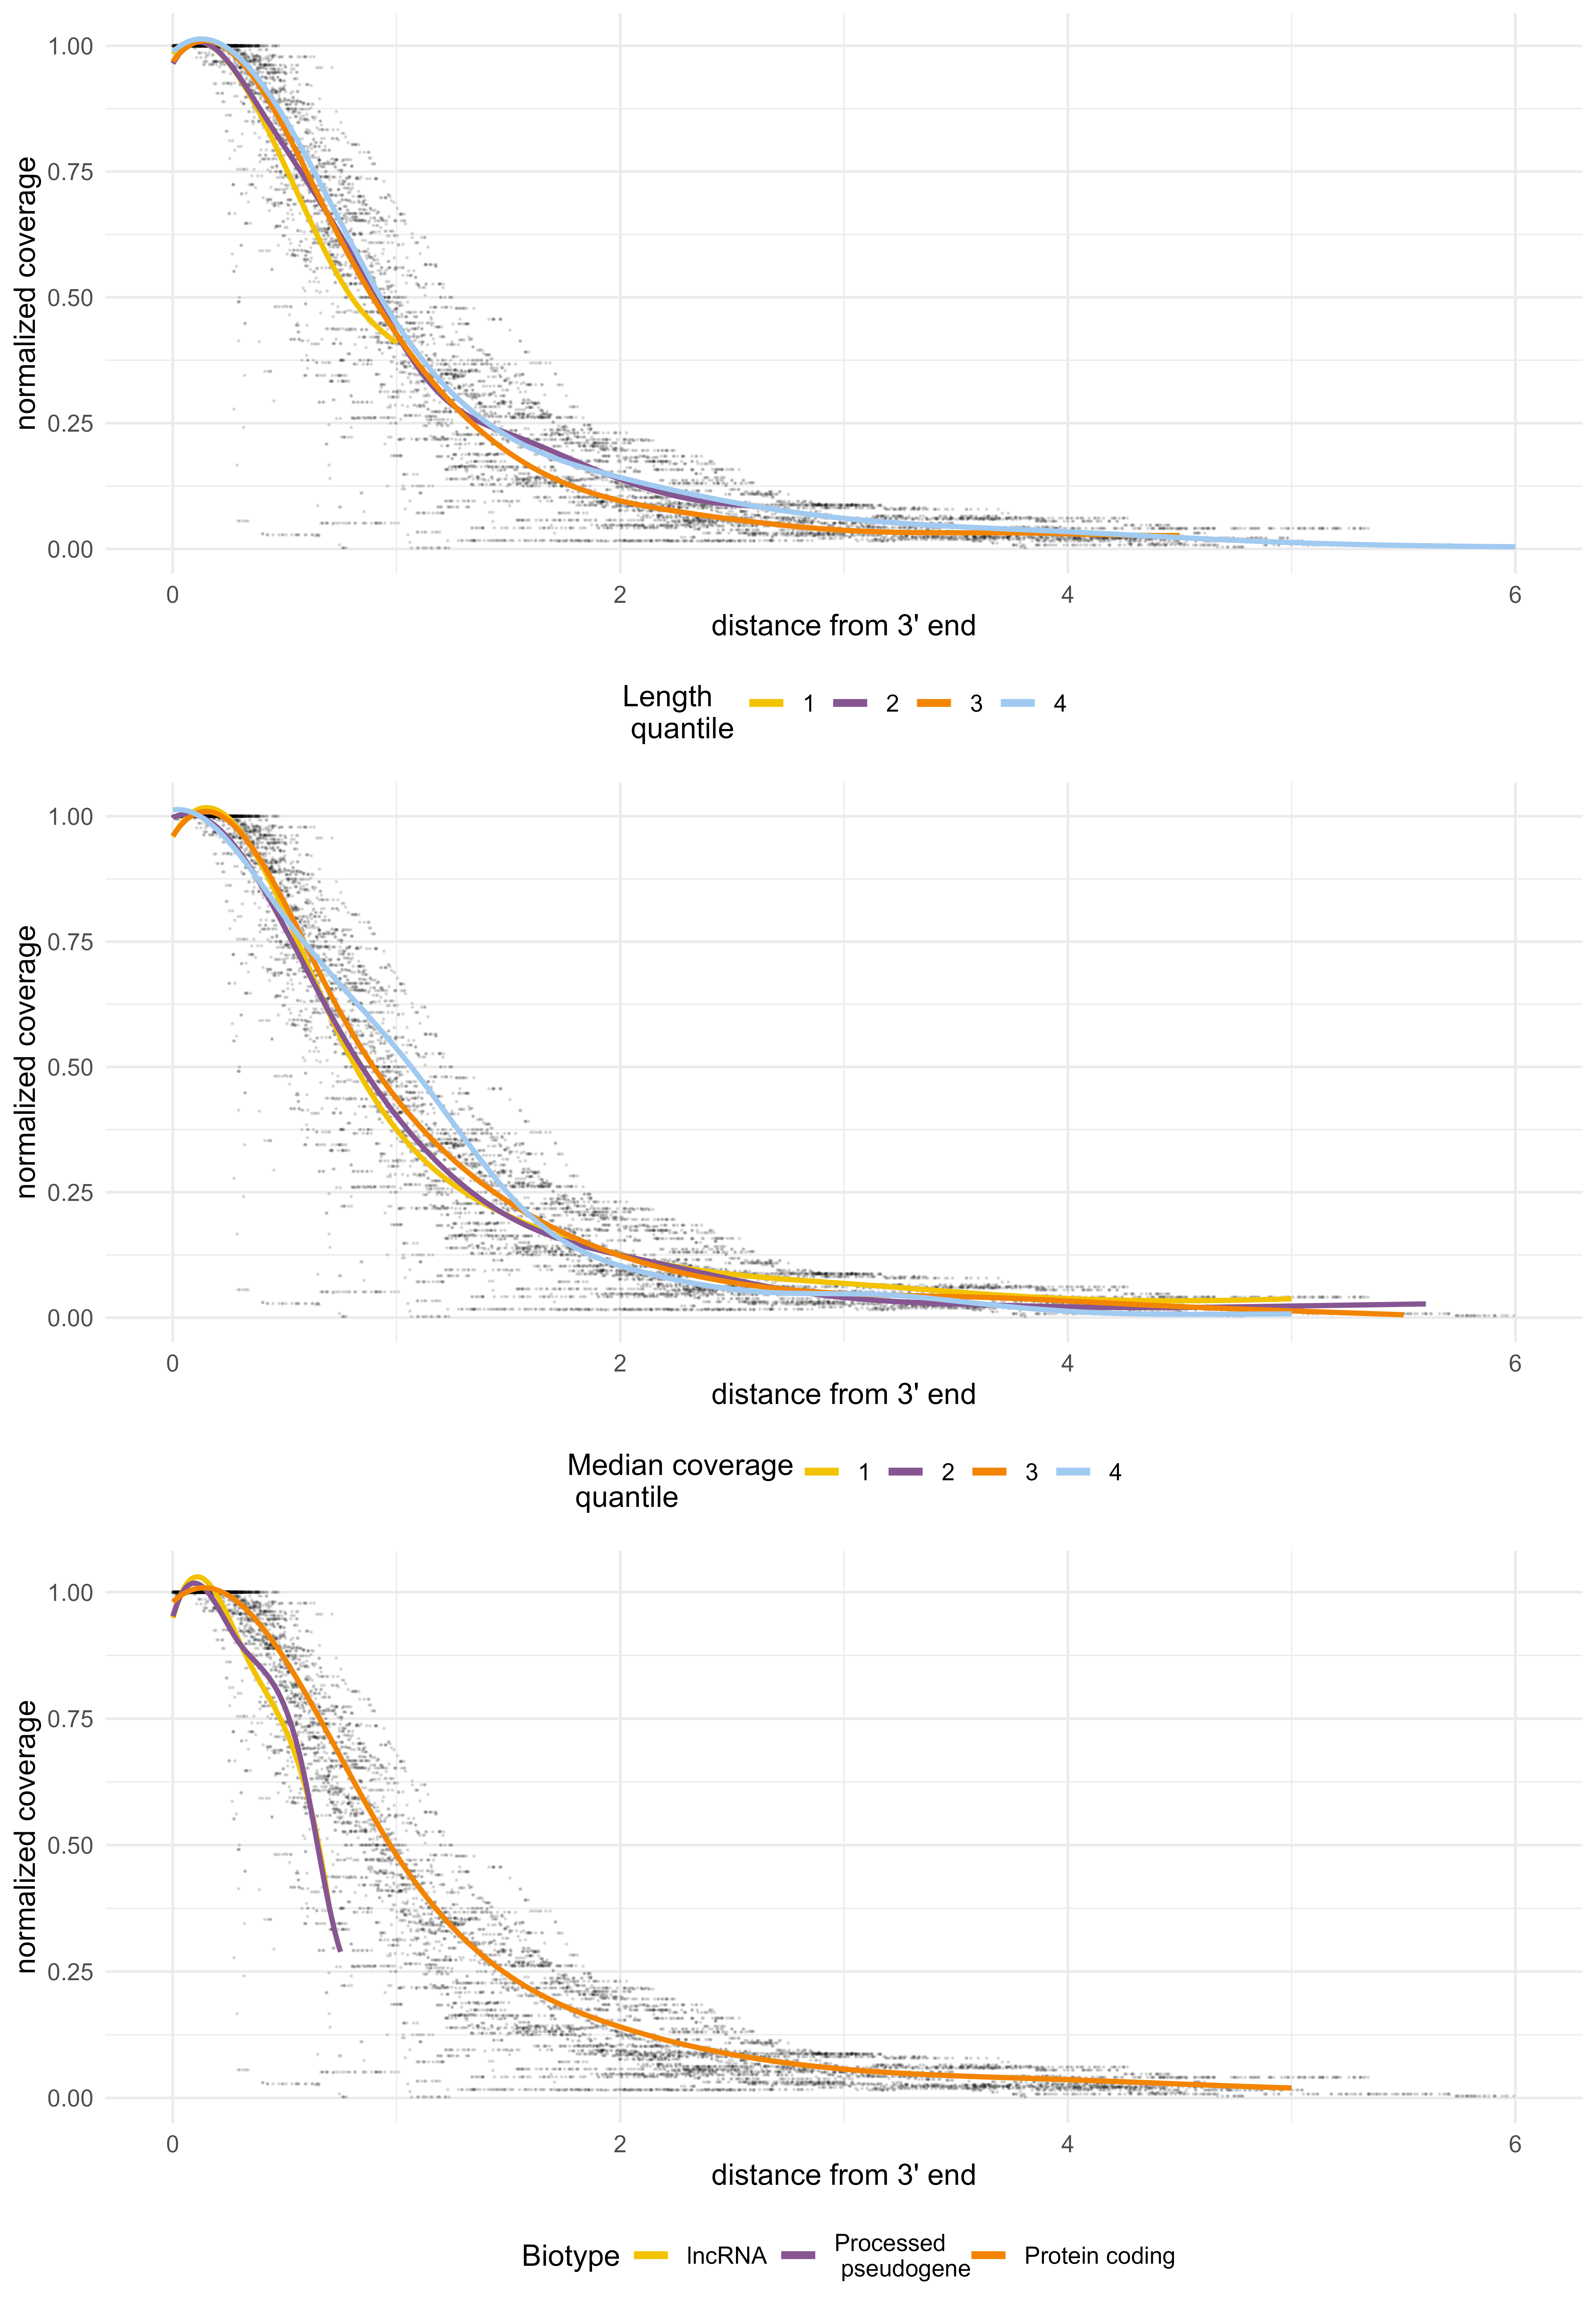
\includegraphics[width=0.95\textwidth]{figures/sec-2-by-feature.png}
    \caption[Degradation curves in MCF7 striated by features]{Degradation curves in MCF7 striated by features. \textbf{a.} Degradation curves fit for isoforms within each length quantile separately, with quantiles at 0\%: 320, 25\%: 1360, 50\%: 2820, 75\%: 5590, 100\%: 9038. \textbf{b.} Degradation curves fit for isoforms within each median coverage quantile separately, with quantiles at 0\%: 7, 25\%: 12, 50\%: 18, 75\%: 31, 100\%: 381. \textbf{c.} Degradation curves fit for isoforms of different biotypes.}
    \label{fig:cov-feature}
\end{figure}

\subsection{Degradation in spike-ins}

We now analyse possible degradation in sequencing spike-ins, which are synthetic RNA molecules added to endogenous RNA samples before library preparation \cite{Lexogen20201}. By doing so, we attempt to elucidate the relative contributions of \textit{in vivo} RNA decay and other extra-cellular factors unrelated to decay, such as library preparation or sequencing artifacts.

We examine SIRVs (Spike-in RNA Variants) \cite{Lexogen20201} present in a subset of SG-NEx samples. Fortunately, a subset of SIRV isoforms are non-overlapping, allowing us to easily apply coverage-based approaches for estimating the degradation. The degradation curves estimated on the SIRVs for six H9 samples (2 runs with 3 replicates each) show consistent patterns amongst themselves (dotted lines, Fig. \ref{fig:cov-spike}), suggesting a constant extraneous factor that acts on degrading SIRV reads. In fact, the degradation rate appears to be constant for each sample, and the average degradation rate is consistent across all samples (run 1: 0.121, 0.148, 0.128; run 2: 0.149, 0.124, 0.183). 

\begin{figure}[H]
    \centering
    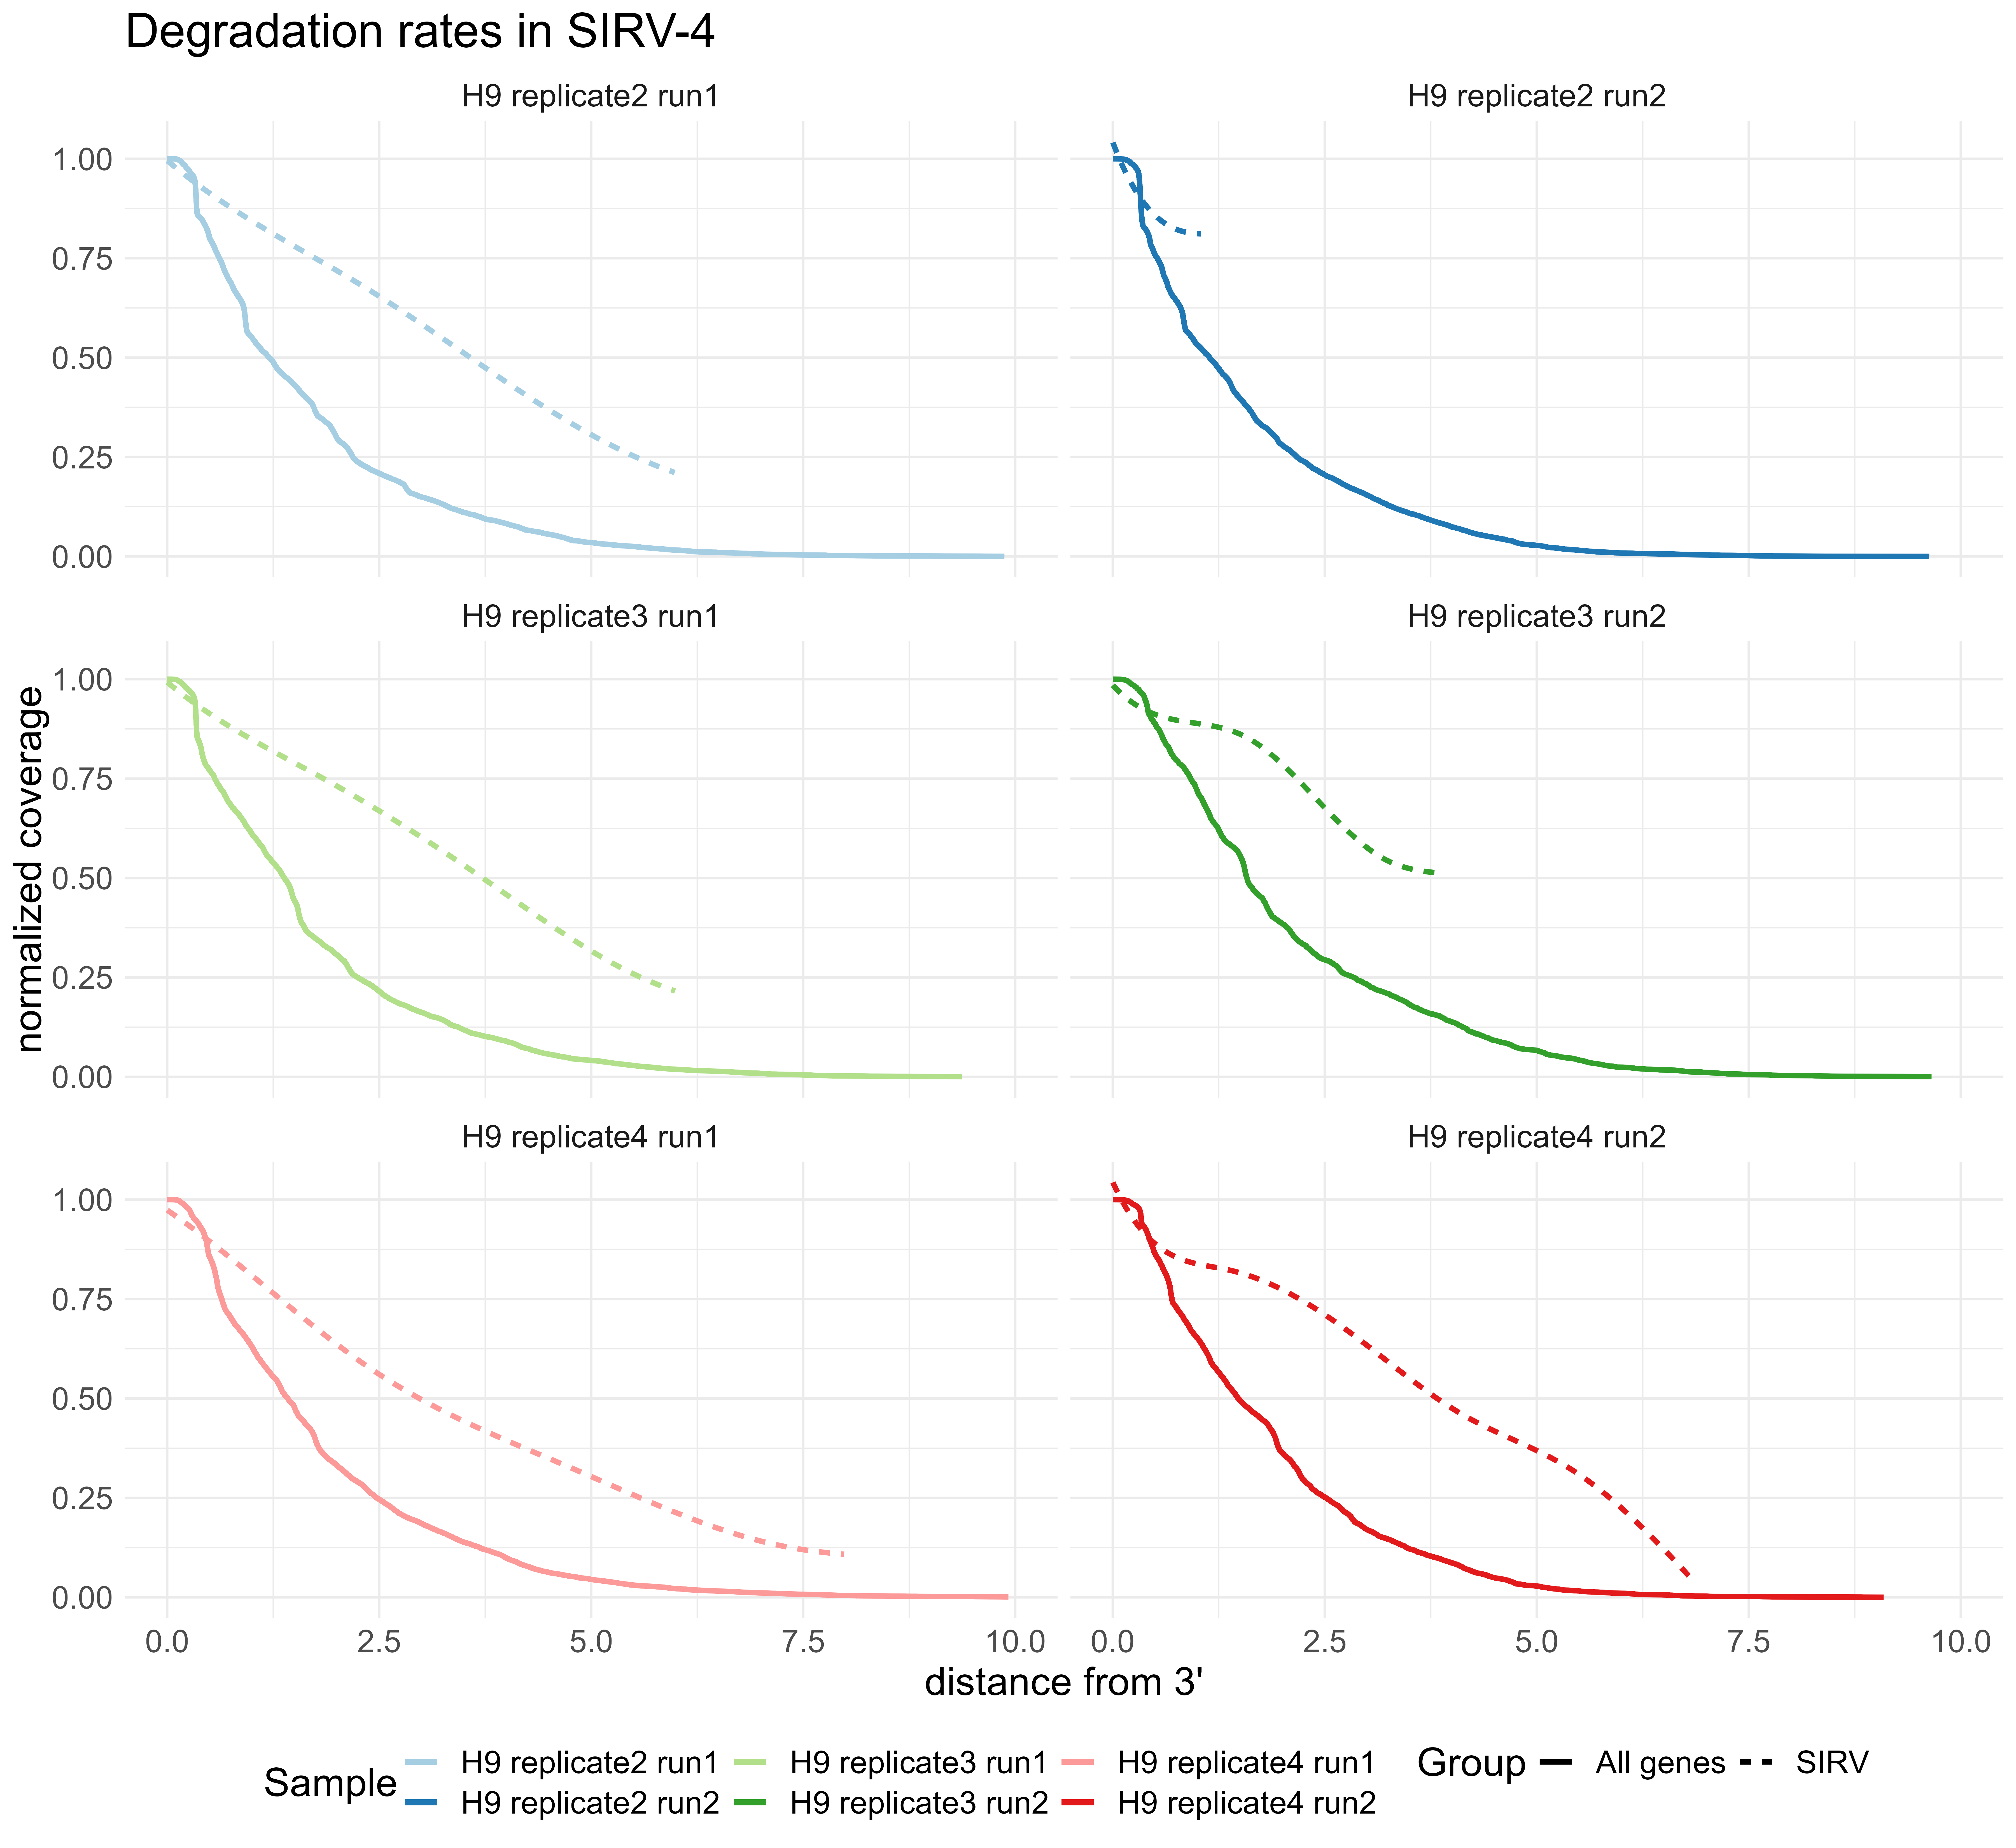
\includegraphics[width=0.9\textwidth]{figures/sec-2-cov-spike.png}
    \caption[Degradation curves for SIRVs based on coverage]{Degradation curves for SIRVs based on coverage for six H9 samples. The number of SIRV transcripts used to fit the degradation curve differs between samples, resulting in curves of different lengths.}
    \label{fig:cov-spike}
\end{figure}

When contrasted against degradation curves estimated on all isoforms from within the same sample (solid lines, Fig. \ref{fig:cov-spike}), the SIRVs show lower rates of degradation. This might suggest that the degradation in endogenous RNAs is a combination of RNA decay \textit{in vivo} and extraneous \textit{in vitro} factors. 

\section{Read length-based degradation estimation}\label{sec:rld}

From the coverage-based estimation of degradation in the preceding sections, we gleaned that patterns of degradation tend to be consistent across transcript isoforms for a given sample across annotated length and median coverage. This holds at least for protein coding isoforms. Based on these observations, we develop a more efficient approach for estimating the degradation rate via the observed read length distributions.

Recall that our objective is to estimate the degradation curve, from which we can easily derive the degradation rate. The key observation for developing a read length-based degradation estimation approach is to note that the degradation curve is essentially the survival function on degraded read lengths. Let $X$ be a random variable denoting the length of a read. Then, its survival function is given by 
\begin{equation}
    S(x)=P(X>x)=1-F(x)
\end{equation}
where $F$ is the cumulative distribution function of $X$. Intuitively, the survival function gives the proportion of reads that exceed (survive after) a given length $x$. We make this clear with an illustration on a hypothetical dataset with a degradation rate of 0.2 (Fig. \ref{fig:survival}). Here, the degradation curve provides an easy way to read off the proportion of degraded reads that are at least 1 kb in length, which is $S(1)=0.8$.   

\begin{figure}[H]
    \centering
    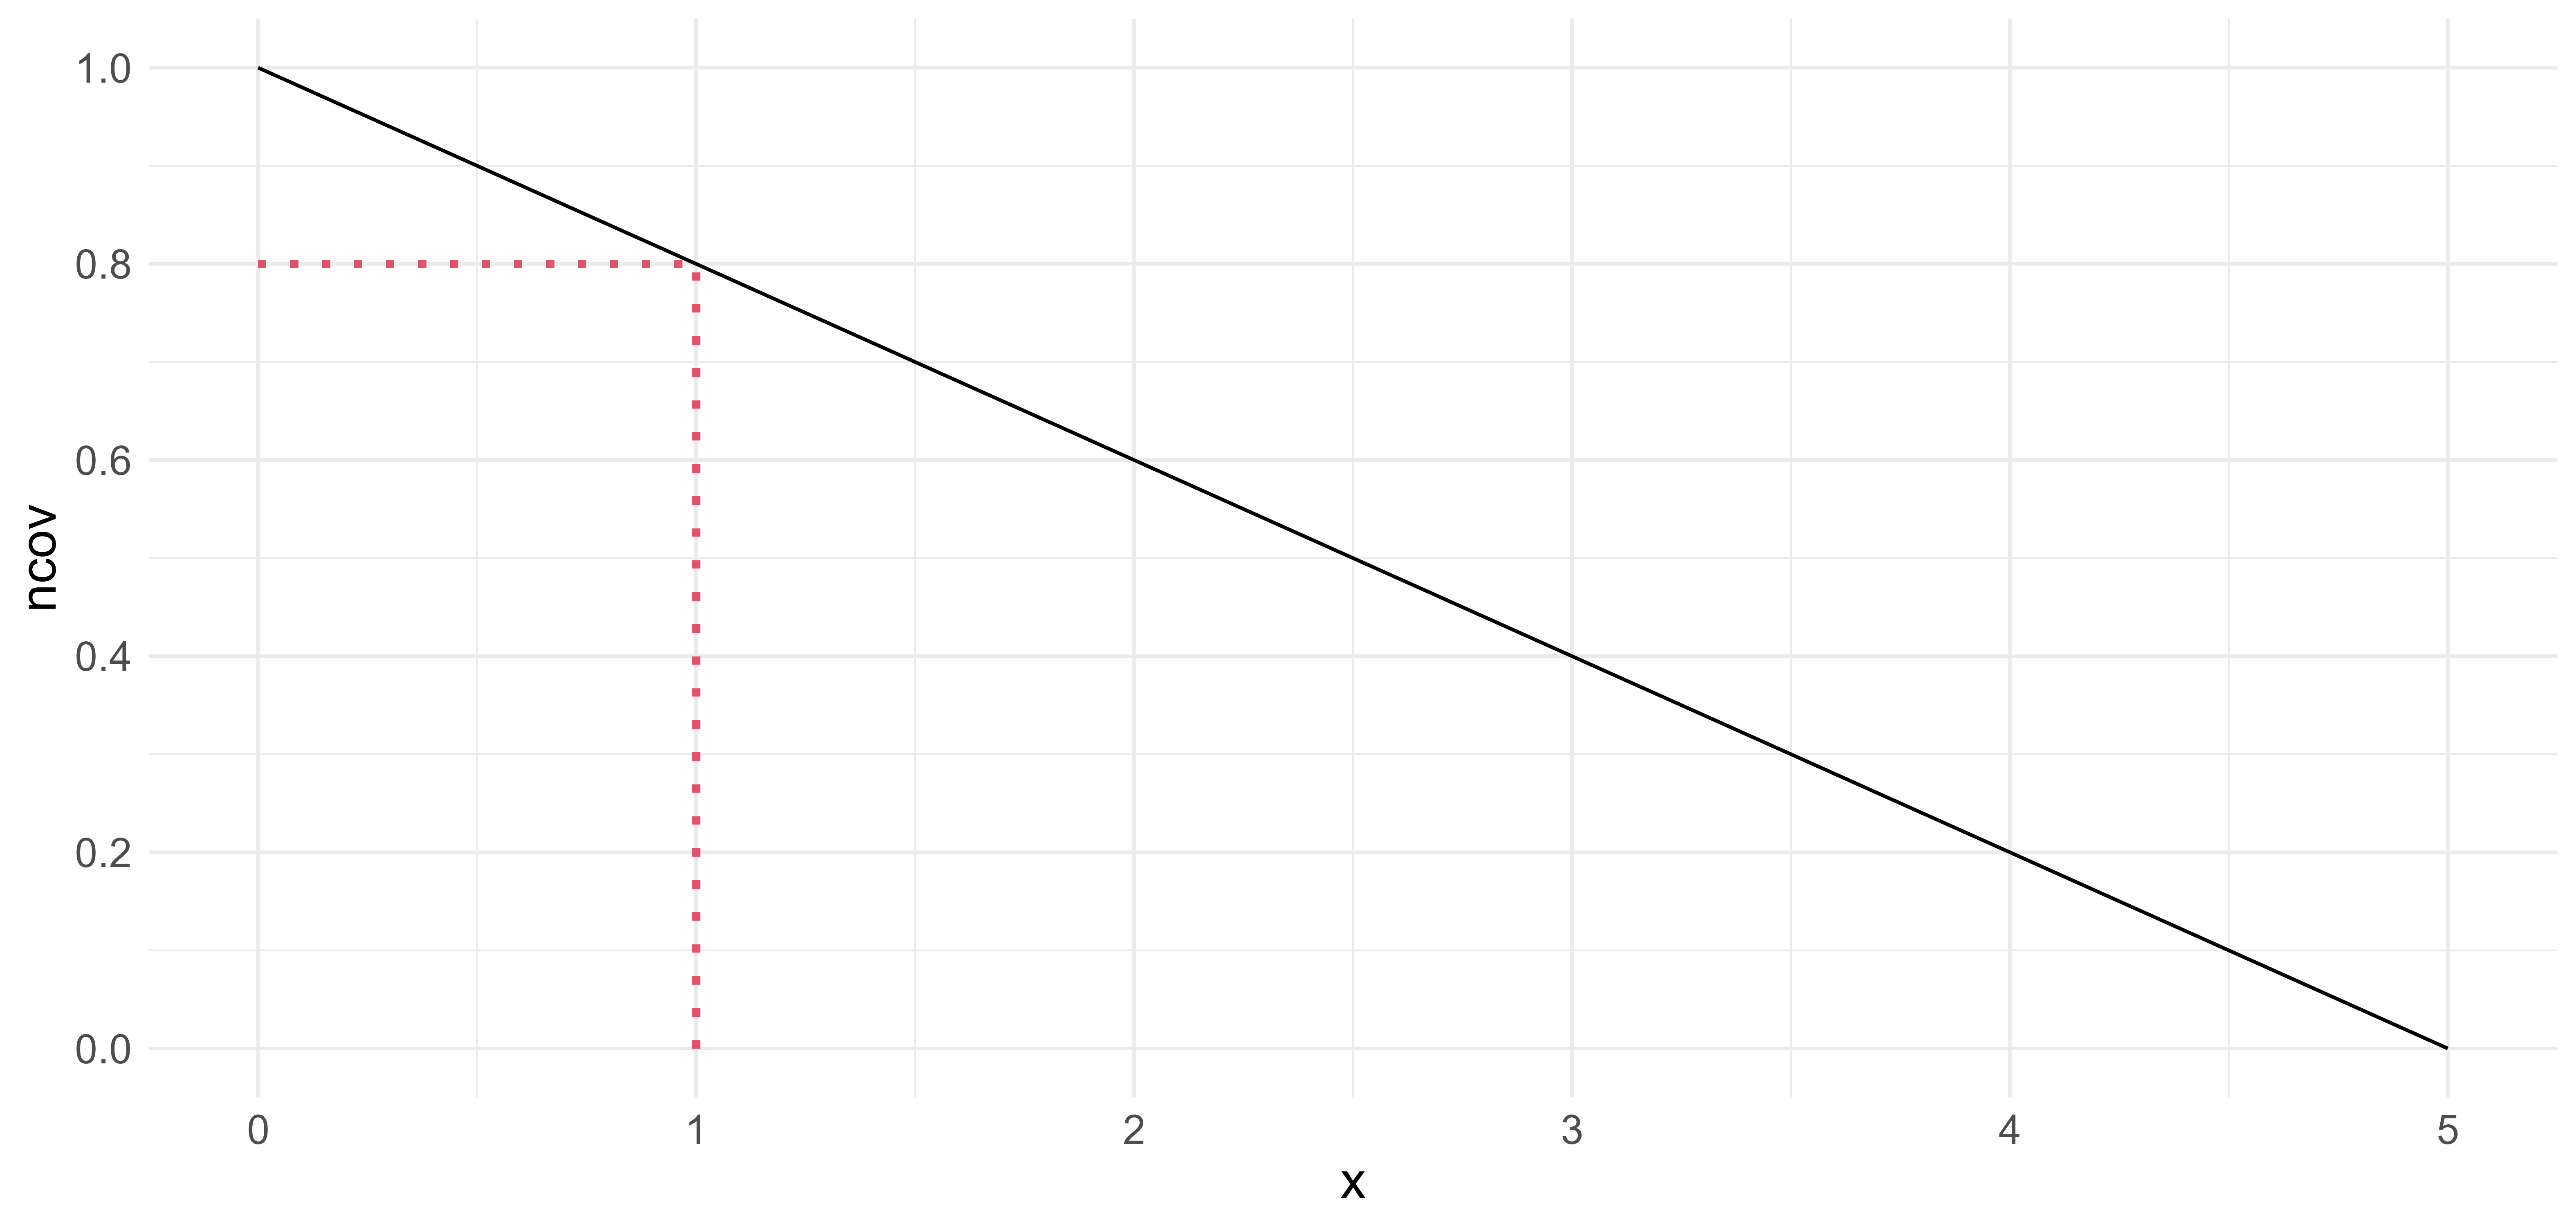
\includegraphics[width=0.85\textwidth]{figures/sec-2-length-example.png}
    \caption[Equivalence between degradation curves and survival functions]{Equivalence between degradation curves and survival functions on degraded read lengths.}
    \label{fig:survival}
\end{figure}

Based on this observation, we develop an approach for estimating degradation based on read length distributions:
\begin{enumerate}
    \item Bin lone isoforms by their length and sample a fixed number of isoforms from each bin. We do so to avoid capturing the isoform length distribution in the degraded read length distribution.  
    \item Extract degraded reads based on the isoforms sampled in step 1. We define degraded reads as those whose lengths are not within the annotated full length by some threshold (in practice, we use 50 bp). 
    \item Compute the empirical cumulative distribution function $F$ on the read lengths obtained in step 2. Deriving the degradation curve $1-F$ is trivial. 
\end{enumerate}

\begin{figure}[H]
    \centering
    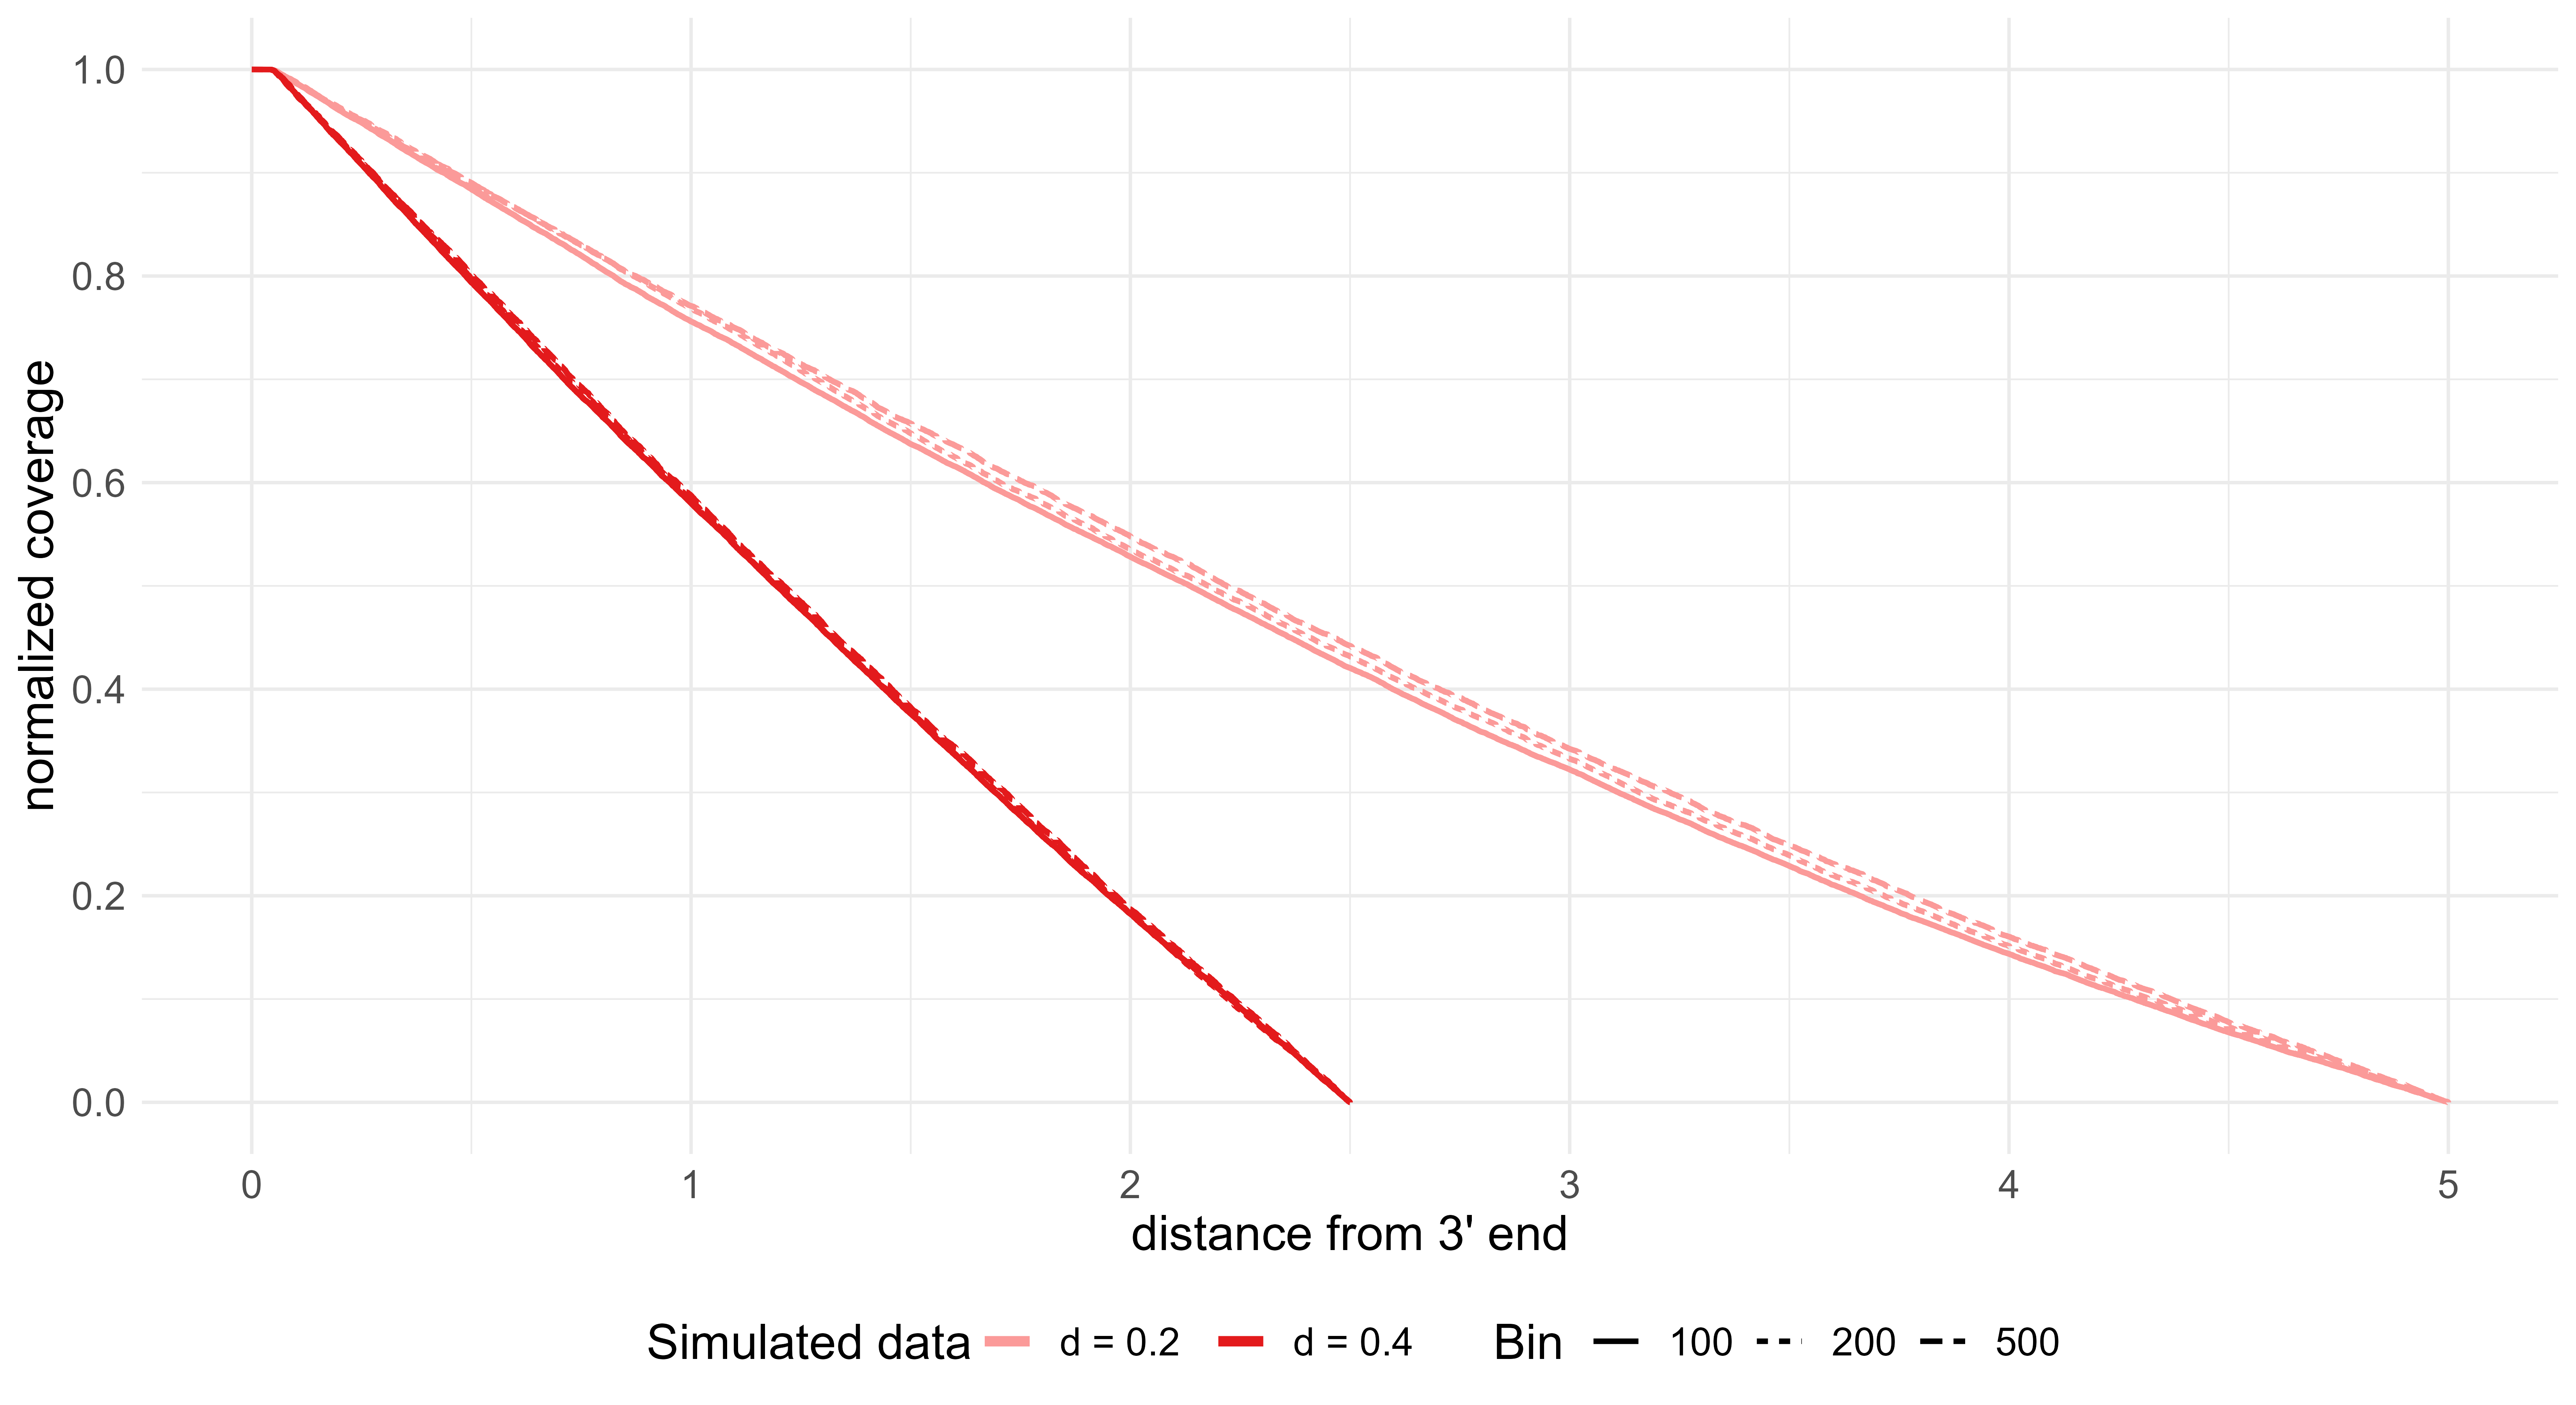
\includegraphics[width=0.85\textwidth]{figures/sec-2-length-sim.png}
    \caption[Degradation curves on simulated datasets based on read length distribution]{Degradation curves on simulated datasets based on read length distribution. For degradation rate of 0.2, coverage drops to 0 at 5 kb (light red), while for degradation rate of 0.4, coverage drops to 0 at 2.5 kb (dark red). The degradation rates are relatively robust to bin size.}
    \label{fig:length-sim}
\end{figure}

\begin{table}[H]
  \centering
    \resizebox{0.45\columnwidth}{!}{%
    \begin{tabular}{|p{3.5cm}|p{1.5cm}|p{1.5cm}|p{1.5cm}|}
\cline{2-4}    \multicolumn{1}{r|}{} & \multicolumn{3}{c|}{Bin size} \bigstrut\\
    \hline
    Simulated dataset & 100   & 200   & 500 \bigstrut\\
    \hline
    d = 0.1 & 0.118 & 0.113 & \textbf{0.107} \bigstrut\\
    \hline
    d = 0.2 & 0.207 & 0.206 & \textbf{0.204} \bigstrut\\
    \hline
    d = 0.4 & \textbf{0.408} & 0.409 & \textbf{0.408} \bigstrut\\
    \hline
    d = 0.5 & 0.513 & 0.512 & \textbf{0.511} \bigstrut\\
    \hline
    \end{tabular}%
    }
  \caption[Degradation estimates on simulated datasets based on read length distribution]{Degradation estimates on simulated datasets based on read length distribution. The length bin size is varied for 100, 200 and 500 bp, and the average degradation rate is computed.}
  \label{tab:binsize}%
\end{table}%

We validate this approach on the same simulated datasets with degradation rates of 0.2 and 0.4 and test the robustness of the length bin size used. The degradation curves qualitatively reflect the expected degradation rate (Fig. \ref{fig:length-sim}) and appear robust to the bin size chosen (Table \ref{tab:binsize}). We note that in the range of bin sizes we tested, a larger bin size yielded estimates closest to the expected degradation rates. Intuitively, a smaller bin size captures more variance in the degraded read length distribution, making the estimates noisier.         

With this validation in hand, we estimated the degradation curves for 32 direct RNA-seq samples spanning six cell lines and six sequencing runs (Table \ref{tab:six-six}) for multiple bin sizes. We observed similar trends in the degradation across all samples, with low rates of degradation toward the 3' end, followed by a relatively linear segment and tapering of towards the 5' end asymptotically. Within each cell line, the degradation curves were mostly consistent, with the exception of a few outlier samples for H9 and HepG2 (Fig. \ref{fig:length-sgnex-curves}).  

Next, we computed a regression line based on the degradation curve and calculated its gradient as a proxy for the \textit{average degradation rate}. Here, the average degradation rate allows for relative comparisons between samples and acts as a summary statistic. In practice, we do not use these point estimates to correct for degradation bias; rather, the entire degradation curve is used to do so (Section \ref{sec:rlia-emp}).   

We report the average degradation across the samples for multiple bin sizes, and group them by cell line (Fig. \ref{fig:length-sgnex}a) and sequencing run (Fig. \ref{fig:length-sgnex}b). We first observe that the estimated degradation rates are relatively robust to bin size. Next, for certain cell lines, there is high variance in estimates, presumably due to the samples being sequenced in multiple different runs (e.g. Hct116). These observations were paralleled on the level of sequencing runs. It is likely that the combination of sequencing runs and cell lines influence the observed degradation, although fitting a linear model for the average degradation rate did not produce significant results.

Lastly, we computed correlations between the estimated degradation rates with raw sequencing metrics (Fig. \ref{fig:pwcor}). We observed moderate negative correlations between degradation rate and raw sequenced lengths, and weak correlation with sequencing quality. Interestingly, the strongest correlation was achieved with read length standard deviaion (SCC = -0.90). We postulate that higher degradation rates result in a smaller possible range of read lenghts, resulting in lower variance in lengths.

\begin{table}[H]
  \centering
  \resizebox{0.65\columnwidth}{!}{%
    \begin{tabular}{|p{1.5cm}|p{1.5cm}|p{1.5cm}|p{1.5cm}|p{1.5cm}|p{1.5cm}|p{1.5cm}|}
\cline{2-7}    \multicolumn{1}{l|}{} & Run1  & Run2  & Run3  & Run4  & Run5  & Run6 \bigstrut\\
    \hline
    A549  & 4     & 0     & 0     & 0     & 0     & 0 \bigstrut\\
    \hline
    H9    & 4     & 3     & 0     & 0     & 0     & 0 \bigstrut\\
    \hline
    Hct116 & 3     & 1     & 2     & 1     & 1     & 1 \bigstrut\\
    \hline
    HepG2 & 3     & 1     & 1     & 0     & 0     & 0 \bigstrut\\
    \hline
    MCF7  & 2     & 1     & 0     & 0     & 0     & 0 \bigstrut\\
    \hline
    K562  & 4     & 0     & 0     & 0     & 0     & 0 \bigstrut\\
    \hline
    \end{tabular}%
    }
      \caption[Description of SG-NEx samples across cell lines and sequencing runs]{Description of SG-NEx samples across cell lines and sequencing runs}
  \label{tab:six-six}%
\end{table}%

\begin{figure}[p]
    \centering
    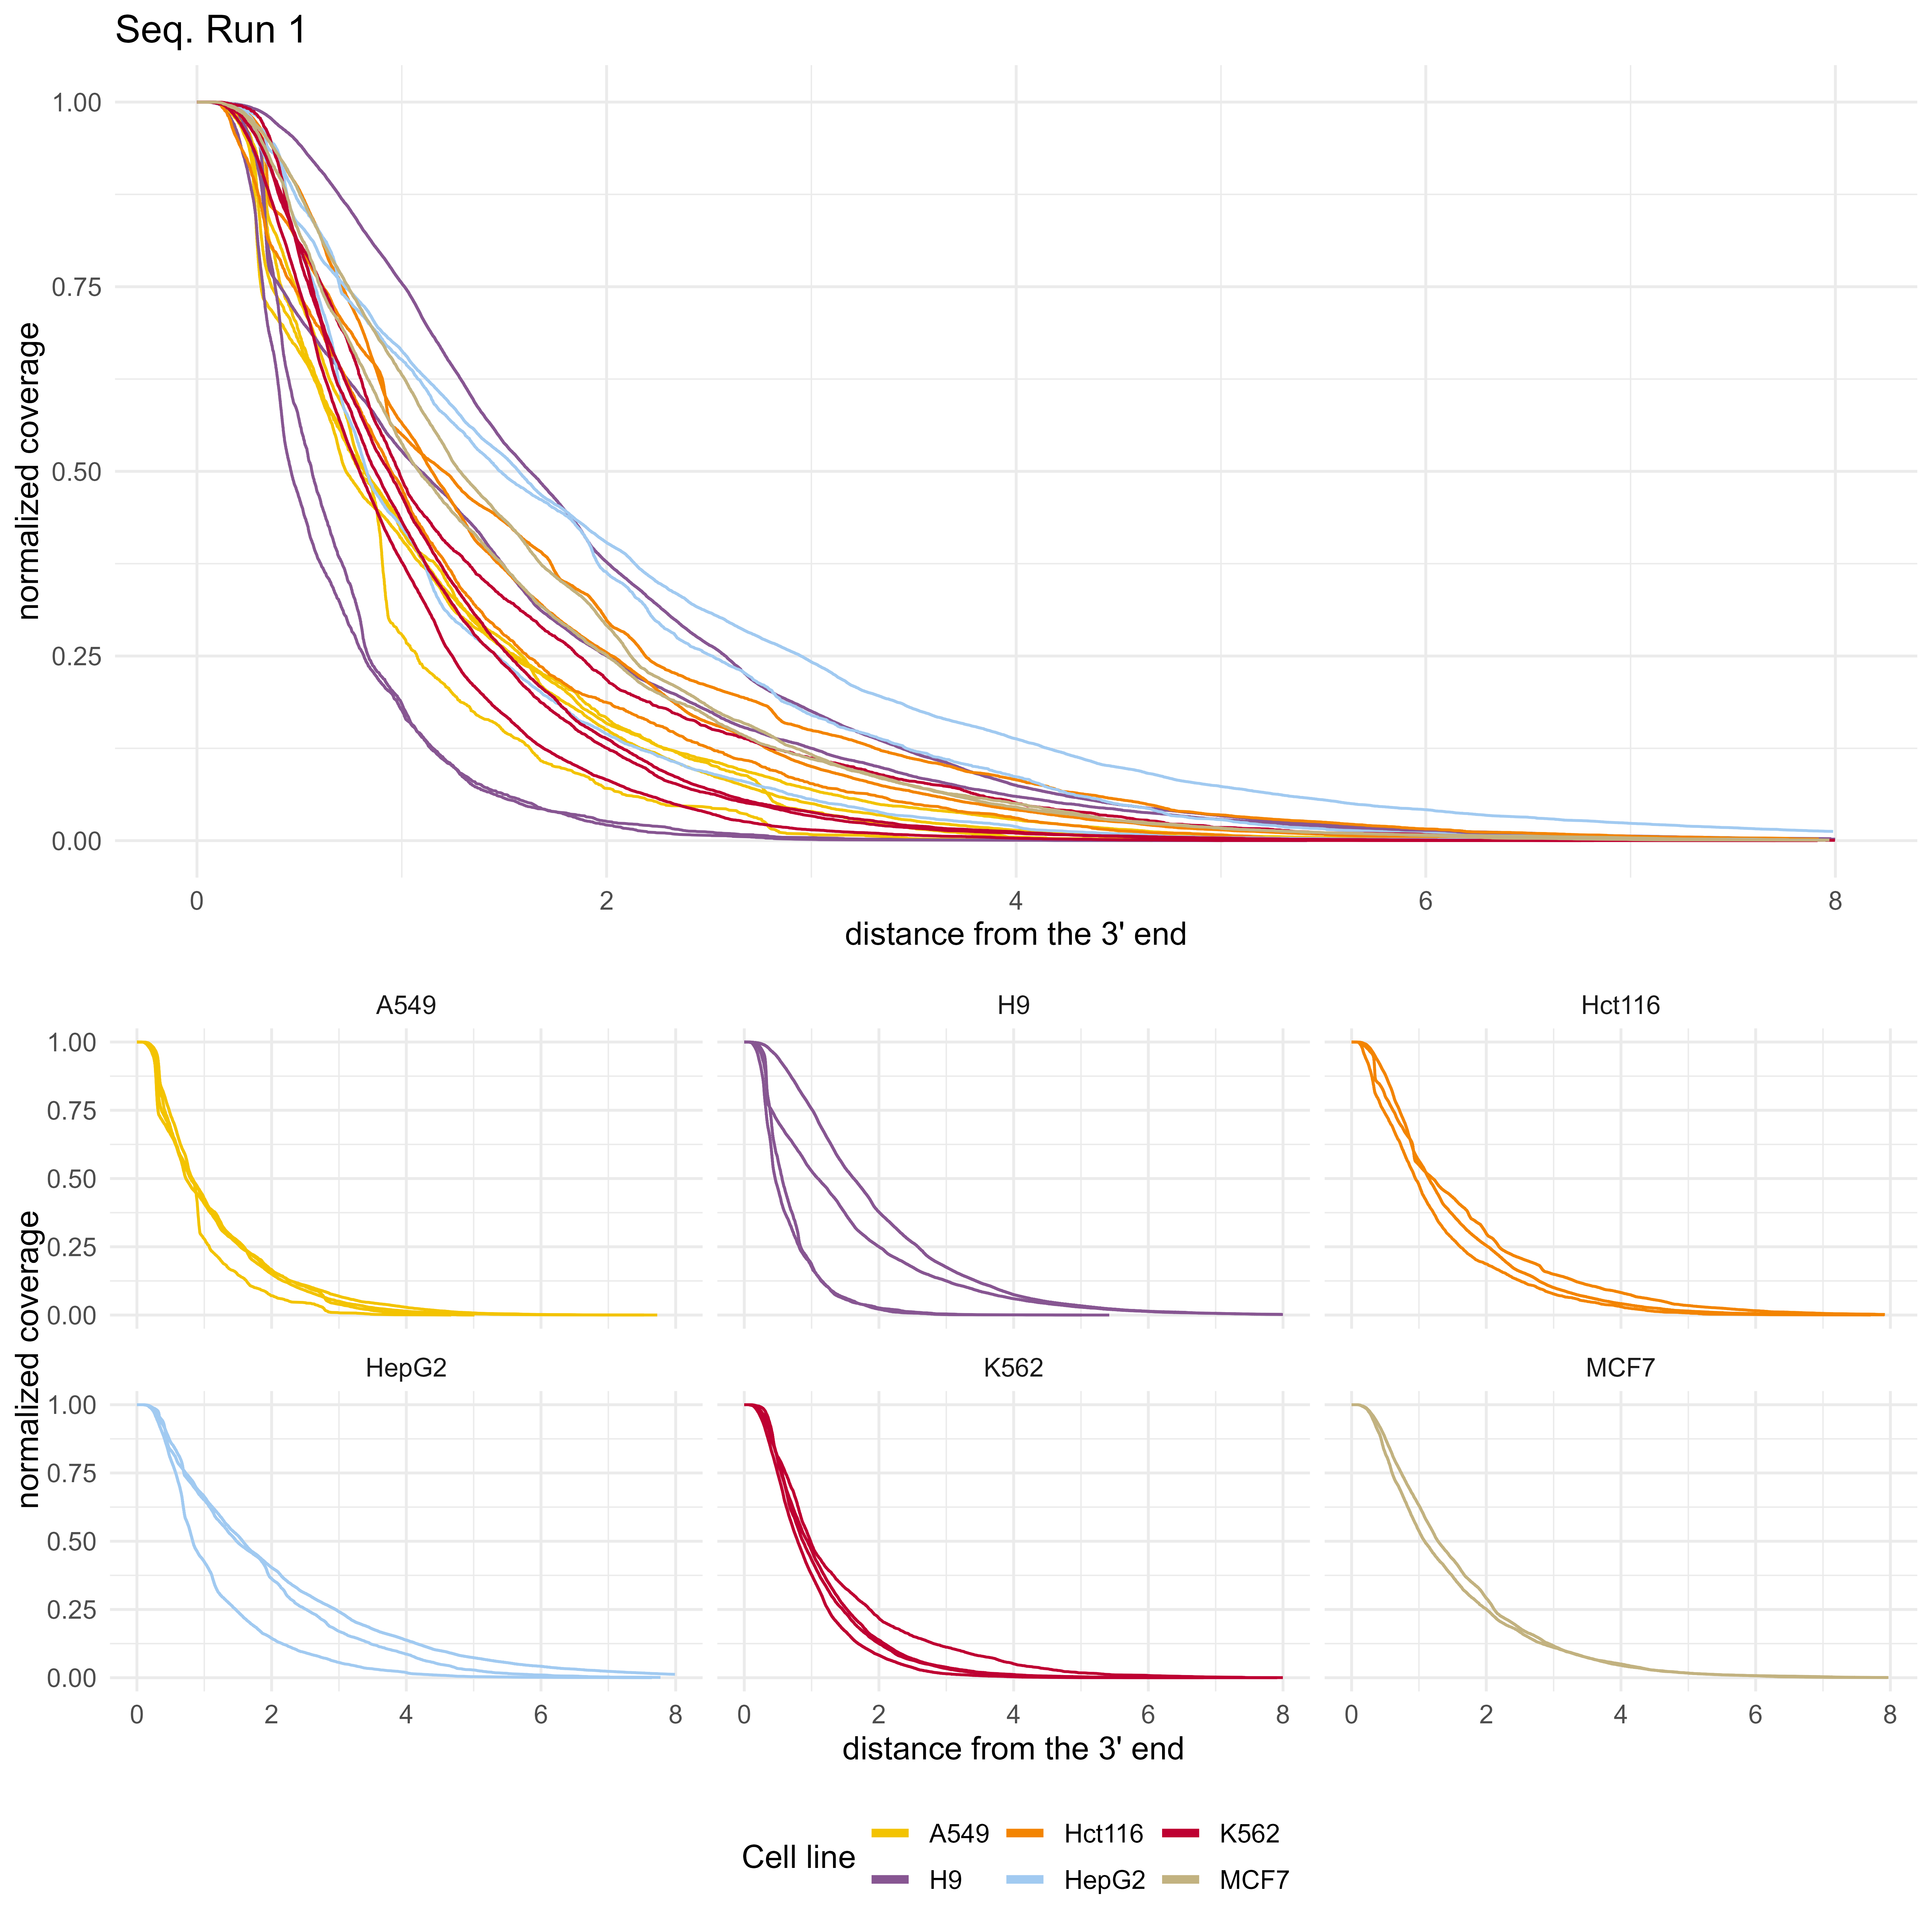
\includegraphics[width=\textwidth]{figures/sec-2-length-sgnex-curves.png}
    \caption[Degradation curves for real datasets based on read length distribution]{Degradation curves for real datasets based on read length distribution for sequencing run 1 with bin size 500. The top panel shows all samples combined. The bottom panel splits the samples by cell lines. In general, the degradation curves show consistent patterns, with low rates of degradation toward the 3' end, followed by a linear segment and a tapering off as distance from the 3' end increases.}
    \label{fig:length-sgnex-curves}
\end{figure}

\begin{figure}[p]
    \centering
    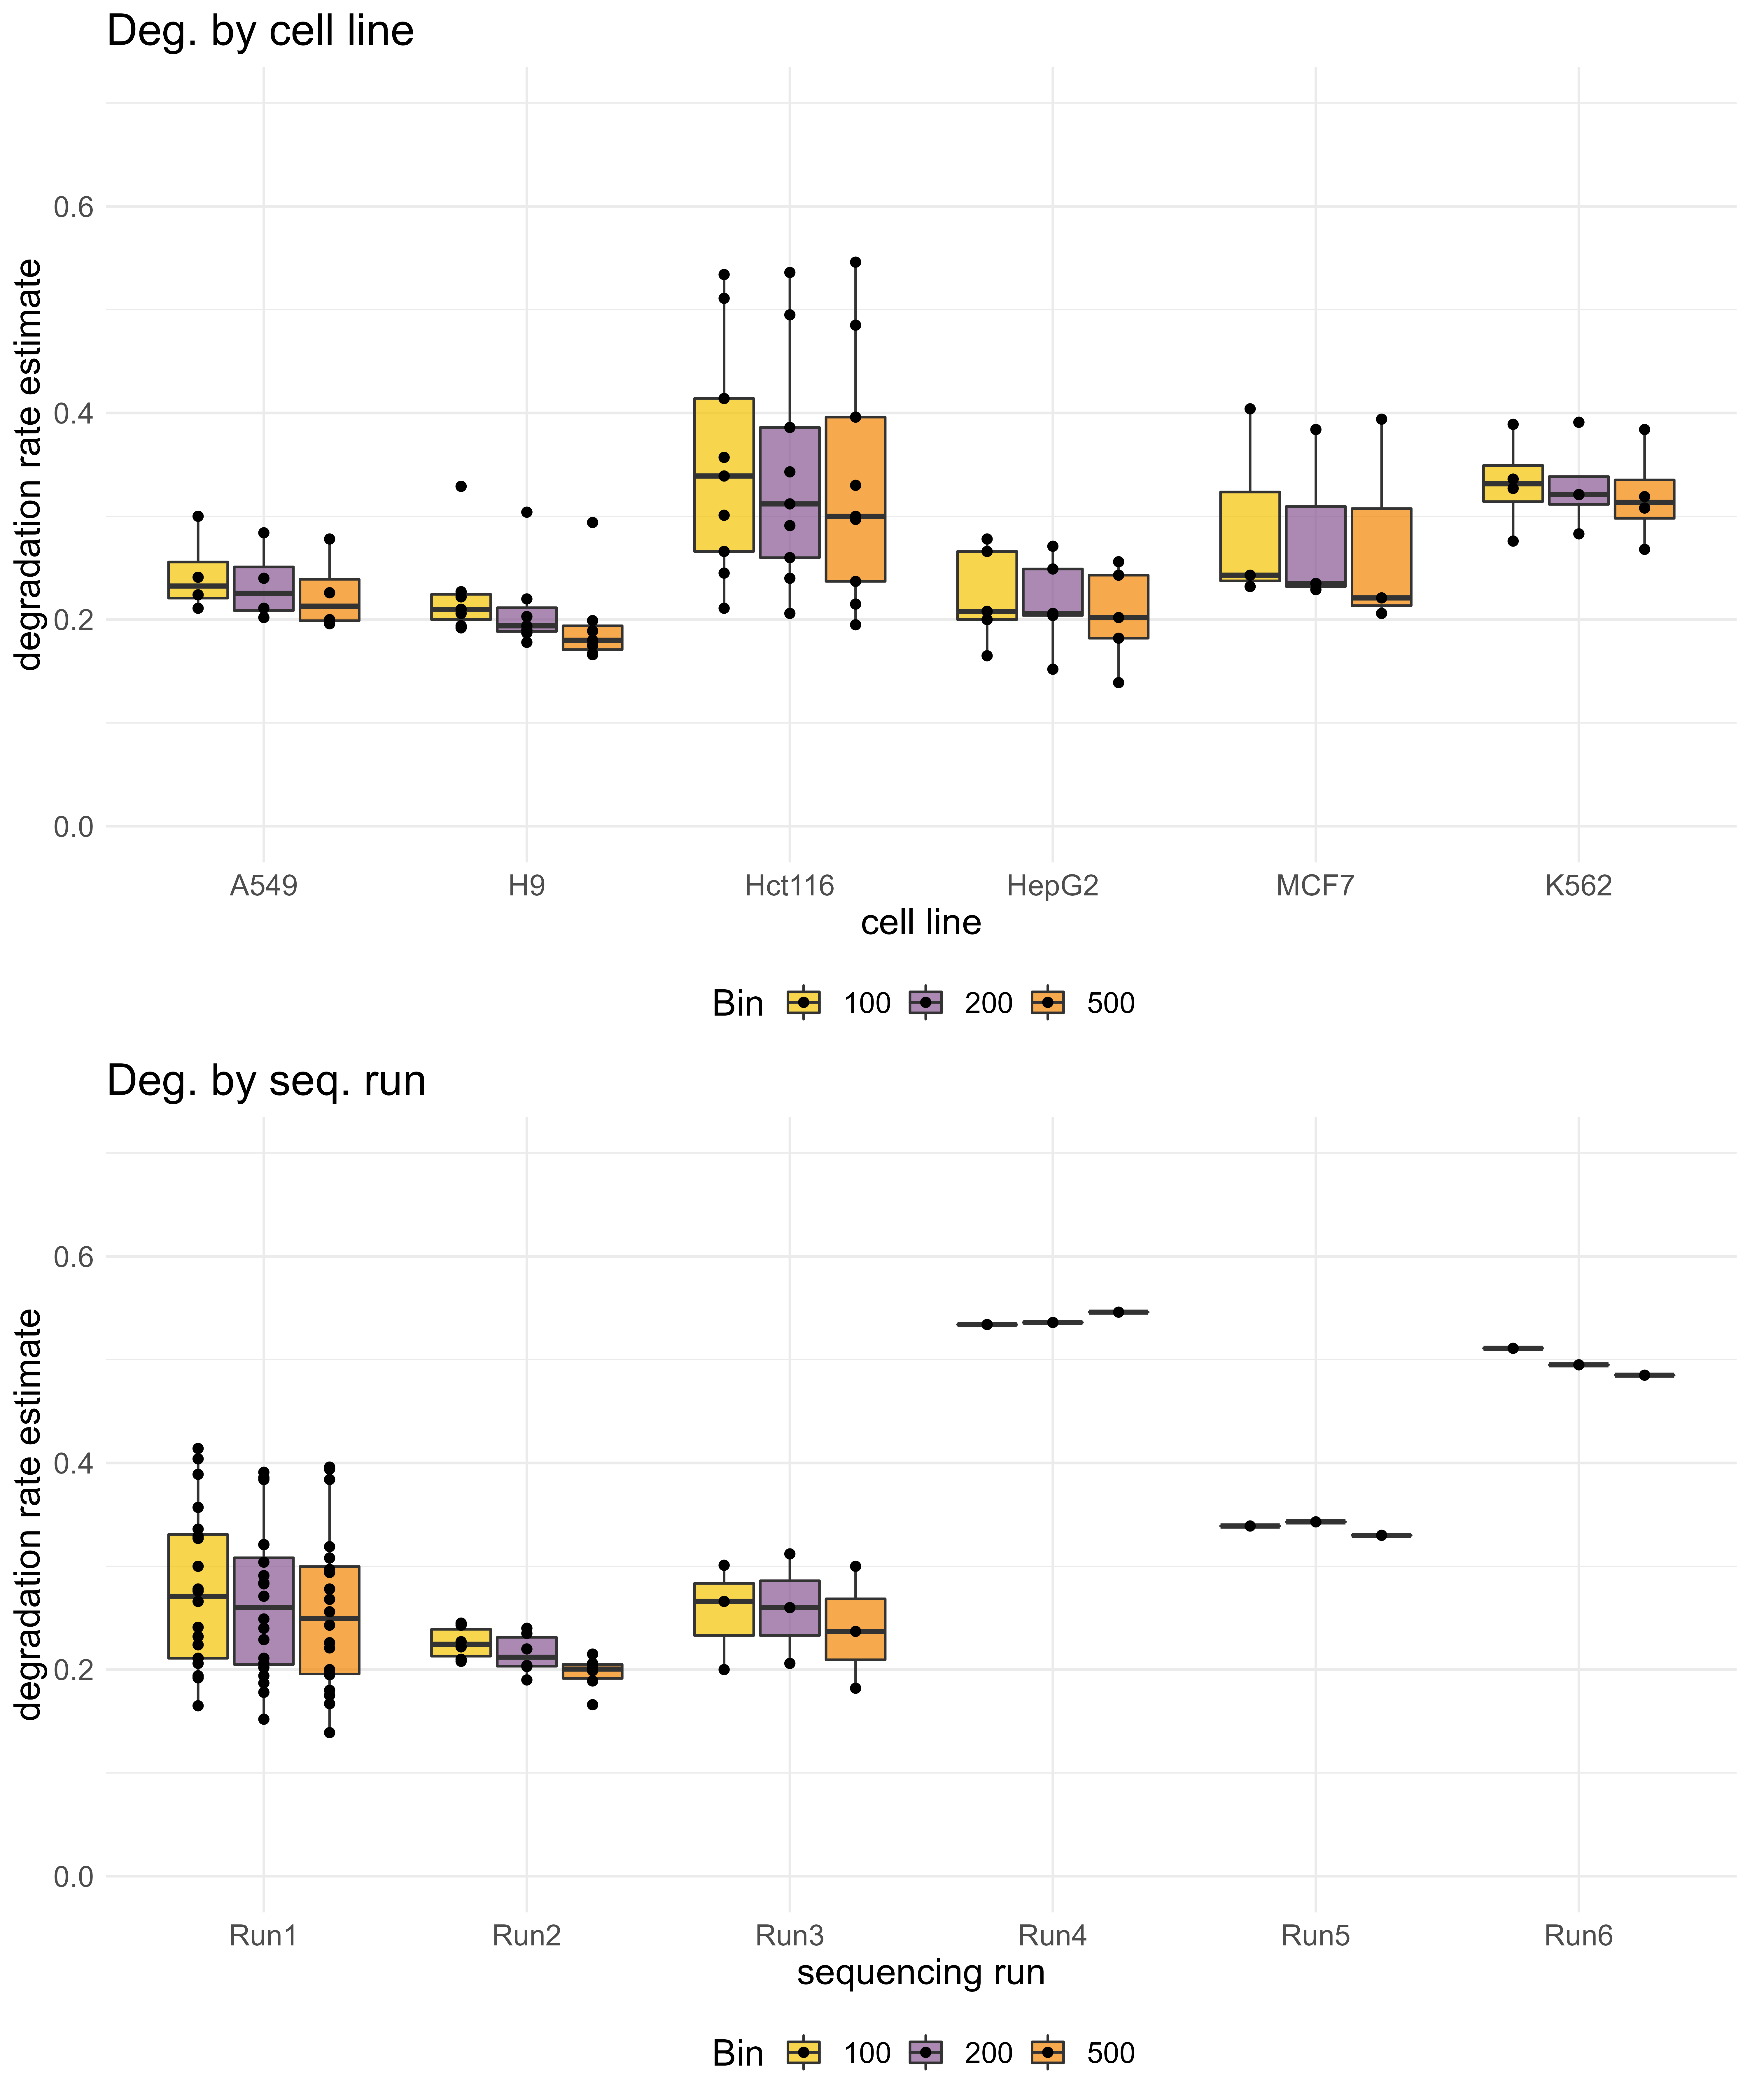
\includegraphics[width=\textwidth]{figures/sec-2-length-sgnex.png}
    \caption[Degradation estimates for real datasets based on read length distribution]{Degradation estimates for real datasets based on read length distribution. The average degradation rate is robust to eh bin size chosen. \textbf{a.} Samples grouped by cell line. \textbf{b.} Samples grouped by sequencing run.}
    \label{fig:length-sgnex}
\end{figure}

\begin{figure}[p]
    \centering
    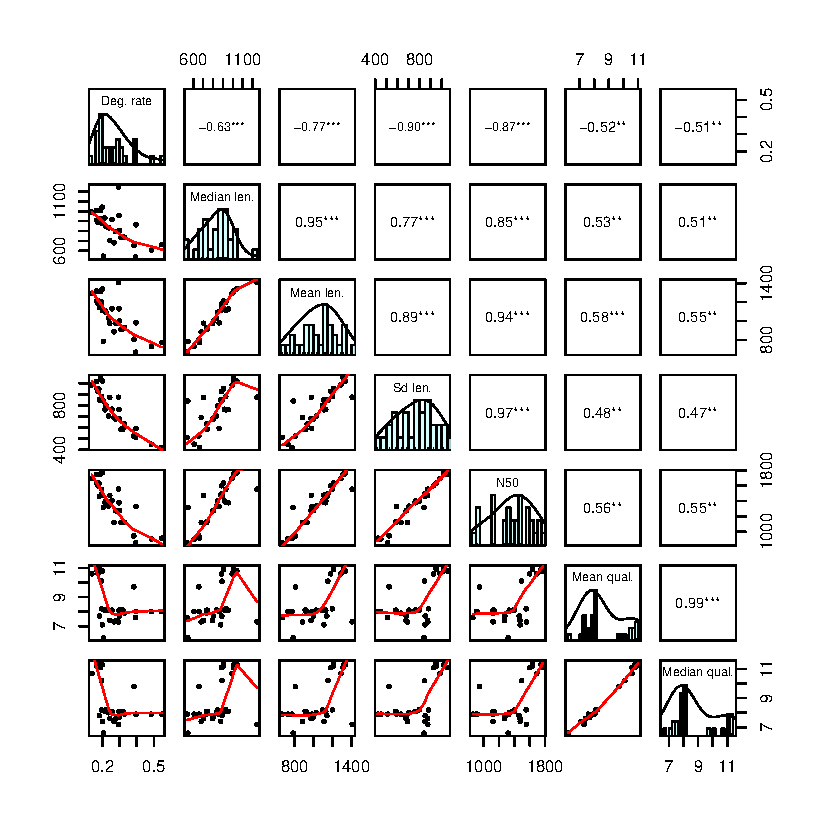
\includegraphics[width=\textwidth]{figures/pwcor.pdf}
    \caption[Correlation of degradation estimates with other sequencing metrics]{Correlation of degradation estimates with other sequencing metrics. From left to right: degradation rate, median length, mean length, read length standard deviation, N50, mean quality and median quality.}
    \label{fig:pwcor}
\end{figure}

\section{Discussion}

In this chapter, we formalized the notion of the degradation rate, and described two approaches for estimating it from long-read direct RNA-seq data. The first approach involves computing the coverage over isoforms and fitting a curve to the coverage track. Based on this approach, we find that degradation curves appear to be mostly consistent across isoforms, and is not dependent on the length of the isoform or the median coverage over the isoform. However, degradation appears to differ by the biotype of the RNA, which corroborates established knowledge. 

Next, we examined the degradation rates in SIRVs and endogenous RNAs from the same samples. SIRV reads exhibited mostly constant degradation rates while endogenous RNAs exhibited variable and steeper degradation rates. This suggests that the observed degradation in endogenous RNA reads is a combination of \textit{in vivo} RNA decay, which contributes a variable component to the degradation, and extraneous \textit{in vitro} factors such as artifacts due to library preparation or sequencing, which contribute a constant component to the degradation. 

Finally, we developed an efficient way of estimating degradation curves based on the degraded read length distribution which does not rely on computing coverage or fitting curves, removing noise and arbitrary parameters in the estimation process. We apply this approach on 32 samples from the SG-NEx project, finding consistent patterns of degradation across all samples. In particular, the degradation curve is flat towards the 3' end, extends into a linear segment and plateaus as distance from the 3' end increases. The low degradation rate observed at the 3' end could be a consequence of protection due to poly(A) tailing and poly(A) binding proteins \textit{in vivo} \cite{Wang2000}. It also suggests that there is a lower bound on the minimum sequence length attainable with ONT sequencing technologies. In the next chapter, we develop a model that uses the estimated degradation curves for bias-aware transcript quantification. 